\documentclass[10pt]{article}
\usepackage[T1]{fontenc}
\usepackage[utf8]{inputenc}
\usepackage[margin=2cm]{geometry}
\usepackage[authoryear,round]{natbib}
\usepackage{amsmath,amssymb,booktabs,graphicx,xcolor,longtable}
\usepackage[hidelinks]{hyperref}
\graphicspath{{figures/}}
% Generated by scripts/paper_lic_rq_v2_assets.py
\newcommand{\nRecords}{11{,}382}
\newcommand{\nTasks}{48}
\newcommand{\nEmptyPrimaries}{6}
\newcommand{\nPermutations}{10{,}000}
\newcommand{\recordsSha}{e313f1ce5985}
\newcommand{\Ktemp}{0.7}
\newcommand{\Krep}{5}
\newcommand{\Lpar}{2}
\newcommand{\maxTok}{2{,}048}
\newcommand{\dialGpt}{0.688}
\newcommand{\freshGpt}{0.896}
\newcommand{\diffGpt}{0.208}
\newcommand{\ciGpt}{[0.063, 0.354]}
\newcommand{\pHolmGpt}{0.026}
\newcommand{\pRawGpt}{0.013}
\newcommand{\dialLlama}{0.854}
\newcommand{\freshLlama}{0.958}
\newcommand{\diffLlama}{0.104}
\newcommand{\ciLlama}{[0.000, 0.208]}
\newcommand{\pHolmLlama}{0.125}
\newcommand{\pRawLlama}{0.125}
\newcommand{\dialMistral}{0.063}
\newcommand{\freshMistral}{0.354}
\newcommand{\diffMistral}{0.292}
\newcommand{\ciMistral}{[0.146, 0.438]}
\newcommand{\pHolmMistral}{0.004}
\newcommand{\pRawMistral}{0.001}
\newcommand{\nFreshOnly}{34}
\newcommand{\nDialOnly}{5}
\newcommand{\crlAuroc}{0.627}
\newcommand{\crlCi}{[0.493, 0.760]}
\newcommand{\crlP}{0.022}
\newcommand{\crlPairs}{687}
\newcommand{\robAllAuroc}{0.571}
\newcommand{\robAllP}{0.057}
\newcommand{\robAllCi}{[0.484, 0.656]}
\newcommand{\robExclAuroc}{0.569}
\newcommand{\robExclP}{0.059}
\newcommand{\robExclCi}{[0.483, 0.655]}
\newcommand{\replayCandidates}{0}
\newcommand{\replaySensCandidates}{0}

% Generated by scripts/paper_merged_cdr_assets.py
\newcommand{\cdrSzeroEDialRange}{0.10--0.14}
\newcommand{\cdrSzeroECtrlRange}{0.82--0.86}
\newcommand{\cdrGptEarly}{0.61}
\newcommand{\cdrGptLate}{0.09}
\newcommand{\cdrGptCtrlLate}{0.64}
\newcommand{\cdrLlamaControlGap}{0.545}
\newcommand{\cdrLlamaControlCiLo}{0.513}
\newcommand{\cdrLlamaControlCiHi}{0.576}
\newcommand{\cdrLlamaControlHolmP}{$<$0.001}
\newcommand{\cdrLlamaControlLateGap}{0.575}
\newcommand{\cdrGemmaControlGap}{0.588}
\newcommand{\cdrGemmaControlCiLo}{0.557}
\newcommand{\cdrGemmaControlCiHi}{0.619}
\newcommand{\cdrGemmaControlHolmP}{$<$0.001}
\newcommand{\cdrGemmaControlLateGap}{0.630}
\newcommand{\cdrLevelMatched}{-0.118}
\newcommand{\cdrLevelMatchedP}{$<$0.001}
\newcommand{\cdrLevelMatchedN}{90}
\newcommand{\cdrLevelMatchedSzeroE}{-0.185}
\newcommand{\ctrlScreenDetect}{0/18}
\newcommand{\earlyCqSignal}{18/18}
\newcommand{\earlyCqNull}{3/12}
\newcommand{\earlyLsSignal}{10/18}
\newcommand{\earlyLsNull}{4/12}
\newcommand{\earlyLsBefore}{7}
\newcommand{\valLlamaDetect}{6/18}
\newcommand{\valLlamaDelay}{29}
\newcommand{\valLlamaLsSignal}{11/18}
\newcommand{\valLlamaLsNull}{6/12}
\newcommand{\valLlamaAggDetect}{3/3}
\newcommand{\valLlamaAggNull}{0/2}
\newcommand{\valGemmaDetect}{1/18}
\newcommand{\valGemmaDelay}{25}
\newcommand{\valGemmaLsSignal}{16/18}
\newcommand{\valGemmaLsNull}{3/12}
\newcommand{\valGemmaAggDetect}{3/3}
\newcommand{\valGemmaAggNull}{1/2}
\newcommand{\replaySsDeltaGpt}{+0.46}
\newcommand{\replaySsDeltaLlama}{+0.42}
\newcommand{\replayLsDeltaGpt}{+0.31}
\newcommand{\silentCQEarly}{0.61}
\newcommand{\silentCQLate}{0.08}
\newcommand{\silentCSEarly}{0.79}
\newcommand{\silentCSLate}{0.64}
\newcommand{\silentLSEarly}{0.54}
\newcommand{\silentLSLate}{0.47}
\newcommand{\silentSSEarly}{0.94}
\newcommand{\silentSSLate}{0.98}
\newcommand{\silentCsSupport}{2976}
\newcommand{\silentRsSupport}{427}
\newcommand{\crlLastGapAuroc}{0.672}
\newcommand{\crlLastGapP}{0.001}
\newcommand{\crlCondAuroc}{0.468}
\newcommand{\crlCondP}{0.674}

\makeatletter
\newcommand{\inputtable}[1]{\@@input #1 }
\makeatother
\renewcommand{\thetable}{S\arabic{table}}
\renewcommand{\thefigure}{S\arabic{figure}}
\renewcommand{\thesection}{S\arabic{section}}

\title{Supplementary Material for\\ ``The Silent Cost of Conversation History in
LLM Reasoning''}
\author{Ali \c{S}enol\\Department of Computer Engineering, Tarsus University}
\date{}

\begin{document}
\sloppy
\maketitle

\noindent This supplement gives design details, audit trails and secondary
results. Each result carries the evidence label defined in the article
(confirmatory, prespecified secondary, exploratory or post hoc); sensitivity
analyses are reported next to frozen results, never in their place. All tables
are generated by scripts in the public repository from hash-checked inputs.

\section{Study 1}

\subsection{Sample, prompts and parsing}
The public math subset of Lost in Conversation has 103 tasks and 585 shards.
Before any model call, eleven tasks were excluded because their normalised
question matched an input of our earlier experiments, and eight because their
shard sequence appeared to alter the problem; two tasks fell into both groups,
leaving 86. A hash-based draw that used no model output selected four
integration tasks, used only to test transport, resumption, parsing, scorers
and plotting, and \nTasks{} science tasks.

The system prompt read: \emph{``Solve incrementally using only information
supplied in this conversation. Prior assistant replies may be wrong and are
not authoritative facts.''} The instruction asked for concise numbered steps
ending with exactly one final line, \texttt{FINAL\_ANSWER: <number>} or
\texttt{STATUS: NEED\_MORE\_INFORMATION}; the two rewordings changed the wording
but not this contract. Both arms received a packed transcript in one user
message. Because the strict final-line parser rejected many replies that did
carry a marker during integration, a semantic-contract parser that still
requires the explicit marker was frozen before the science run; raw responses
and strict scores are retained. Six empty Mistral-7B primaries were kept as
invalid, never retried, and represented in later history by
\texttt{[EMPTY\_PRIMARY\_RESPONSE]}.

\begin{table}[h]\centering\small
\caption{Study 1 primary endpoint restricted to tasks with format-valid final
responses in both arms (sensitivity analysis).}
\label{tab:formatvalid}
\begin{tabular}{lccc}\toprule
Model & Tasks retained & Paired difference & McNemar $p$\\\midrule
\inputtable{generated/table_format_valid.tex}
\bottomrule\end{tabular}\end{table}

\subsection{Cumulative Resolution Lag}
Table~\ref{tab:crl} gives the frozen per-model results. In the post-hoc
persistence check, the last pre-final readiness gap alone reached AUROC
\crlLastGapAuroc{}, and CRL within its strata \crlCondAuroc{}.

\begin{table}[h]\centering\small
\caption{Frozen CRL discrimination of a positive final readiness gap
(confirmatory, auxiliary). Cases/controls: units with and without the target.}
\label{tab:crl}
\resizebox{\linewidth}{!}{%
\begin{tabular}{lcccccc}\toprule
Model & Units & Cases/controls & Mean CRL & AUROC [95\% CI] & $p$ & $p_{\text{Holm}}$\\\midrule
\inputtable{generated/table_crl.tex}
\bottomrule\end{tabular}}\end{table}

\subsection{Per-model metric trajectories}
Figures~\ref{fig:s1gpt}--\ref{fig:s1mistral} show all six dimensions per turn
with their support. Gaps are structurally unobservable values, not zeros.

\begin{figure}[htbp]\centering
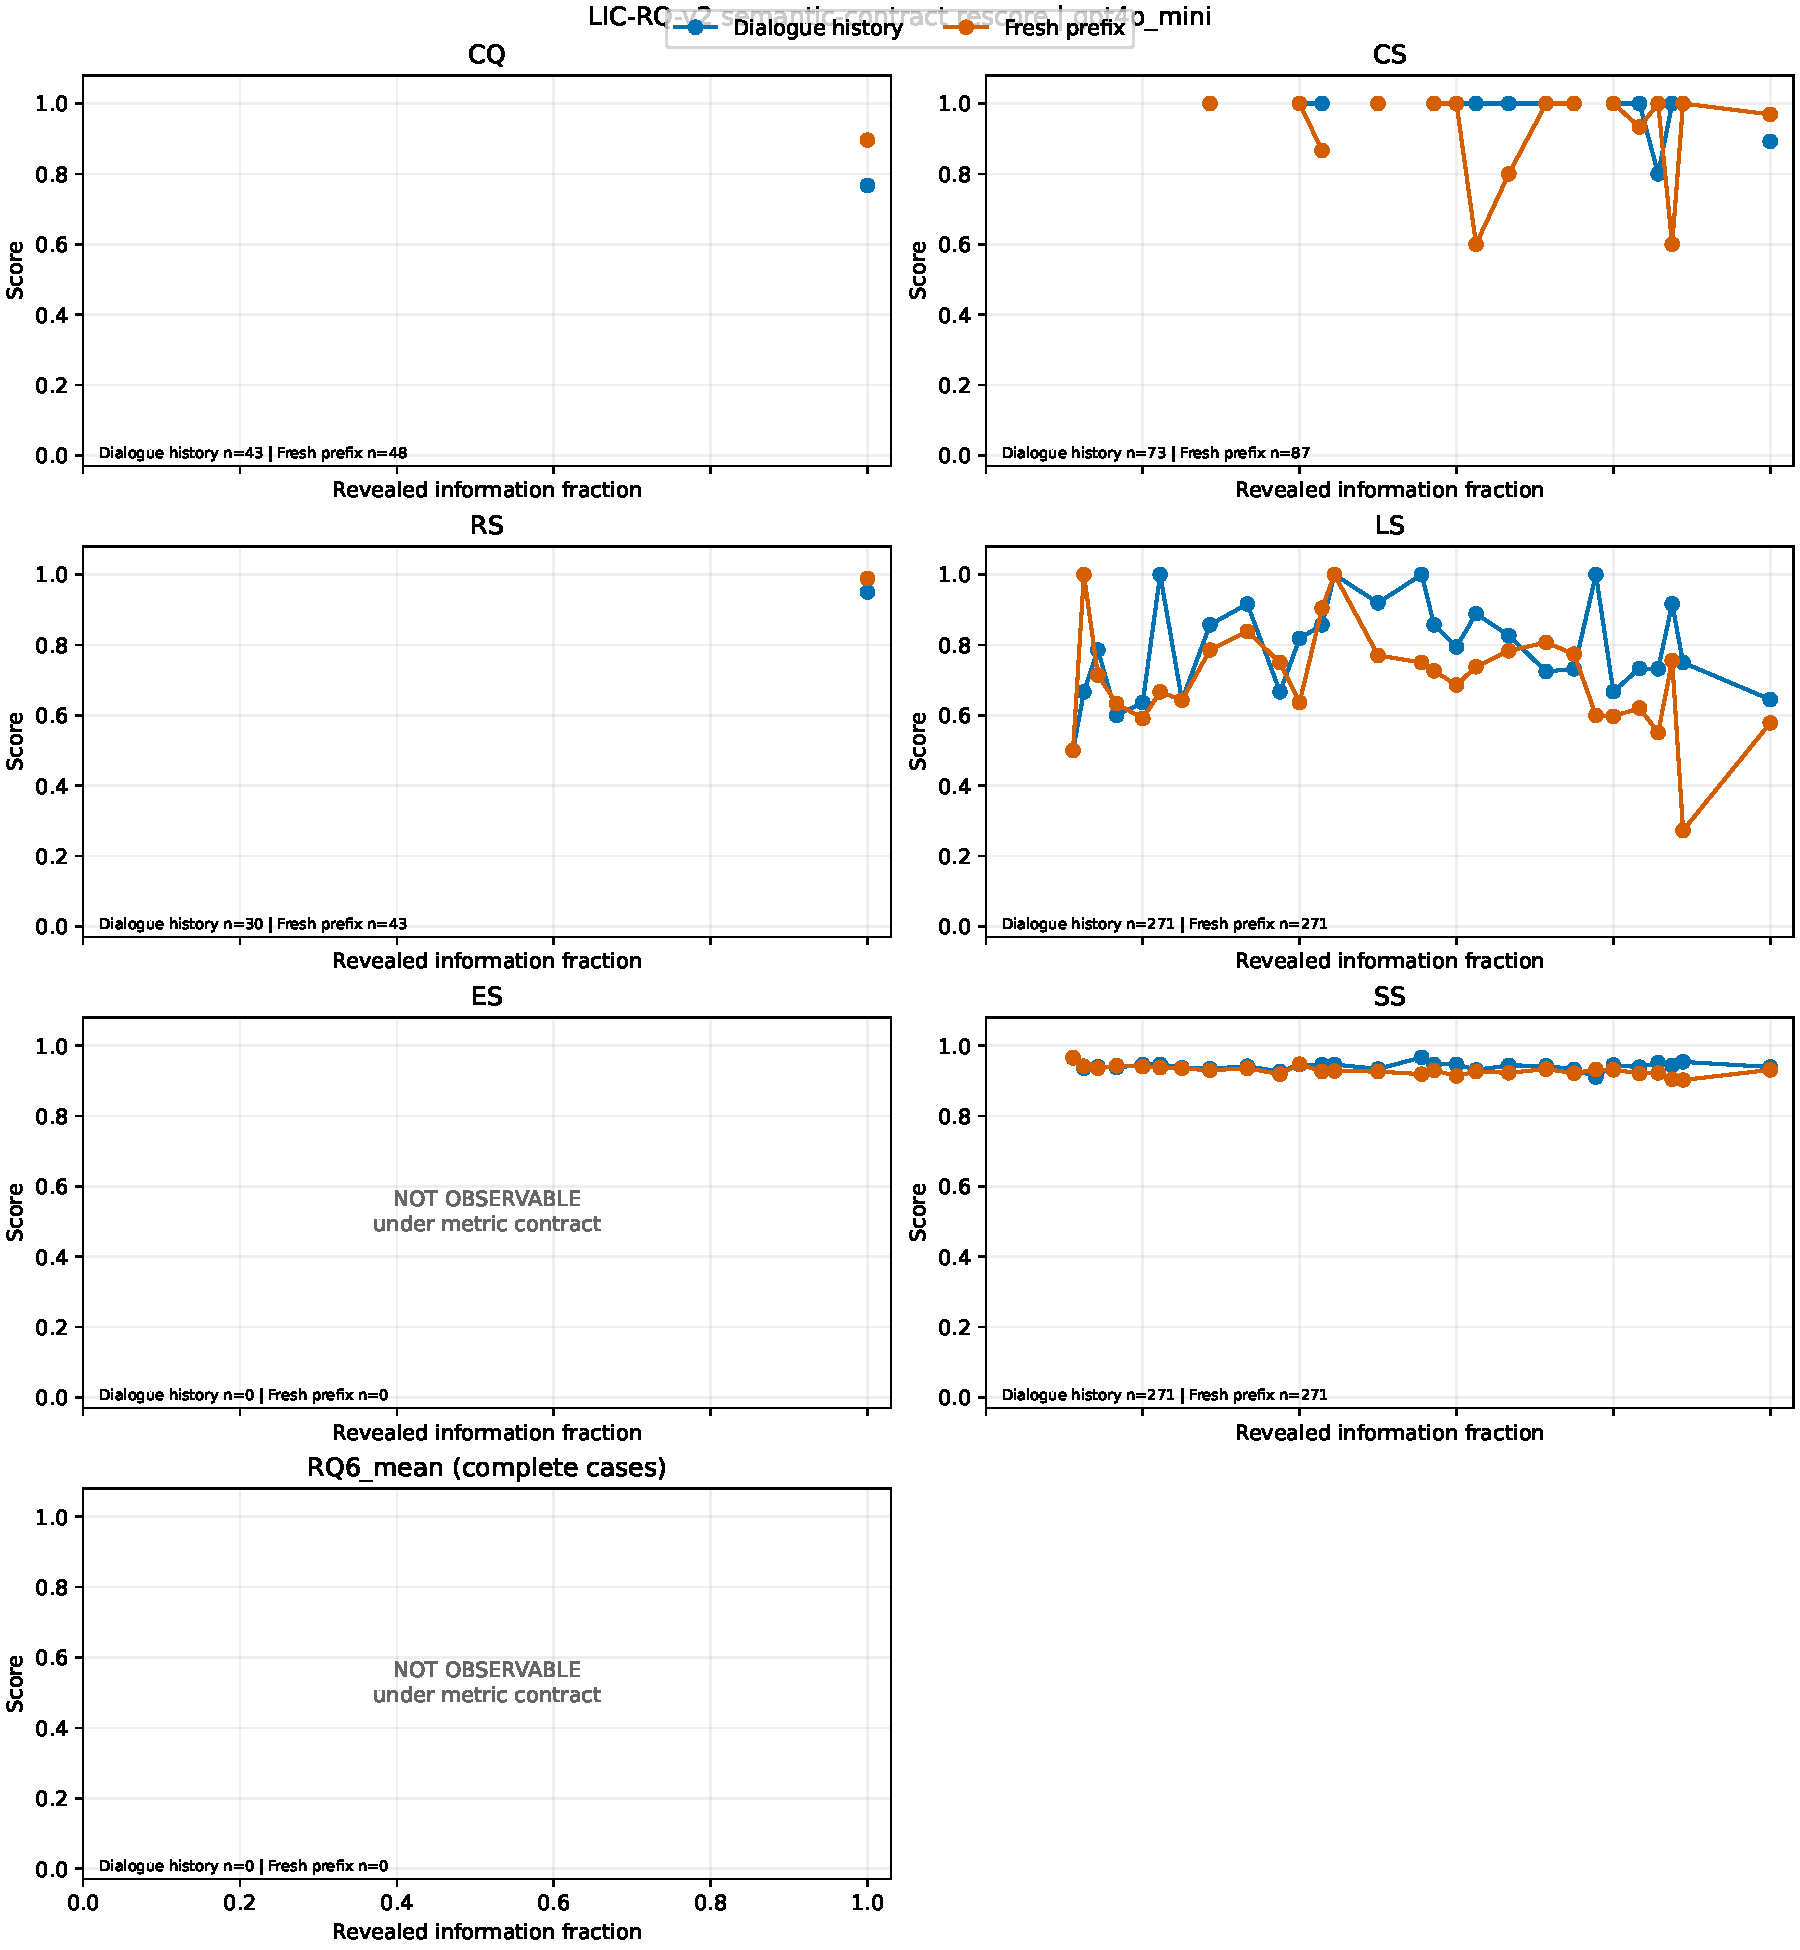
\includegraphics[width=0.85\linewidth]{supp_s1_metrics_gpt4o_mini.pdf}
\caption{Study 1, GPT-4o-mini: per-turn trajectories of the six dimensions and
their complete-case mean.}\label{fig:s1gpt}\end{figure}
\begin{figure}[htbp]\centering
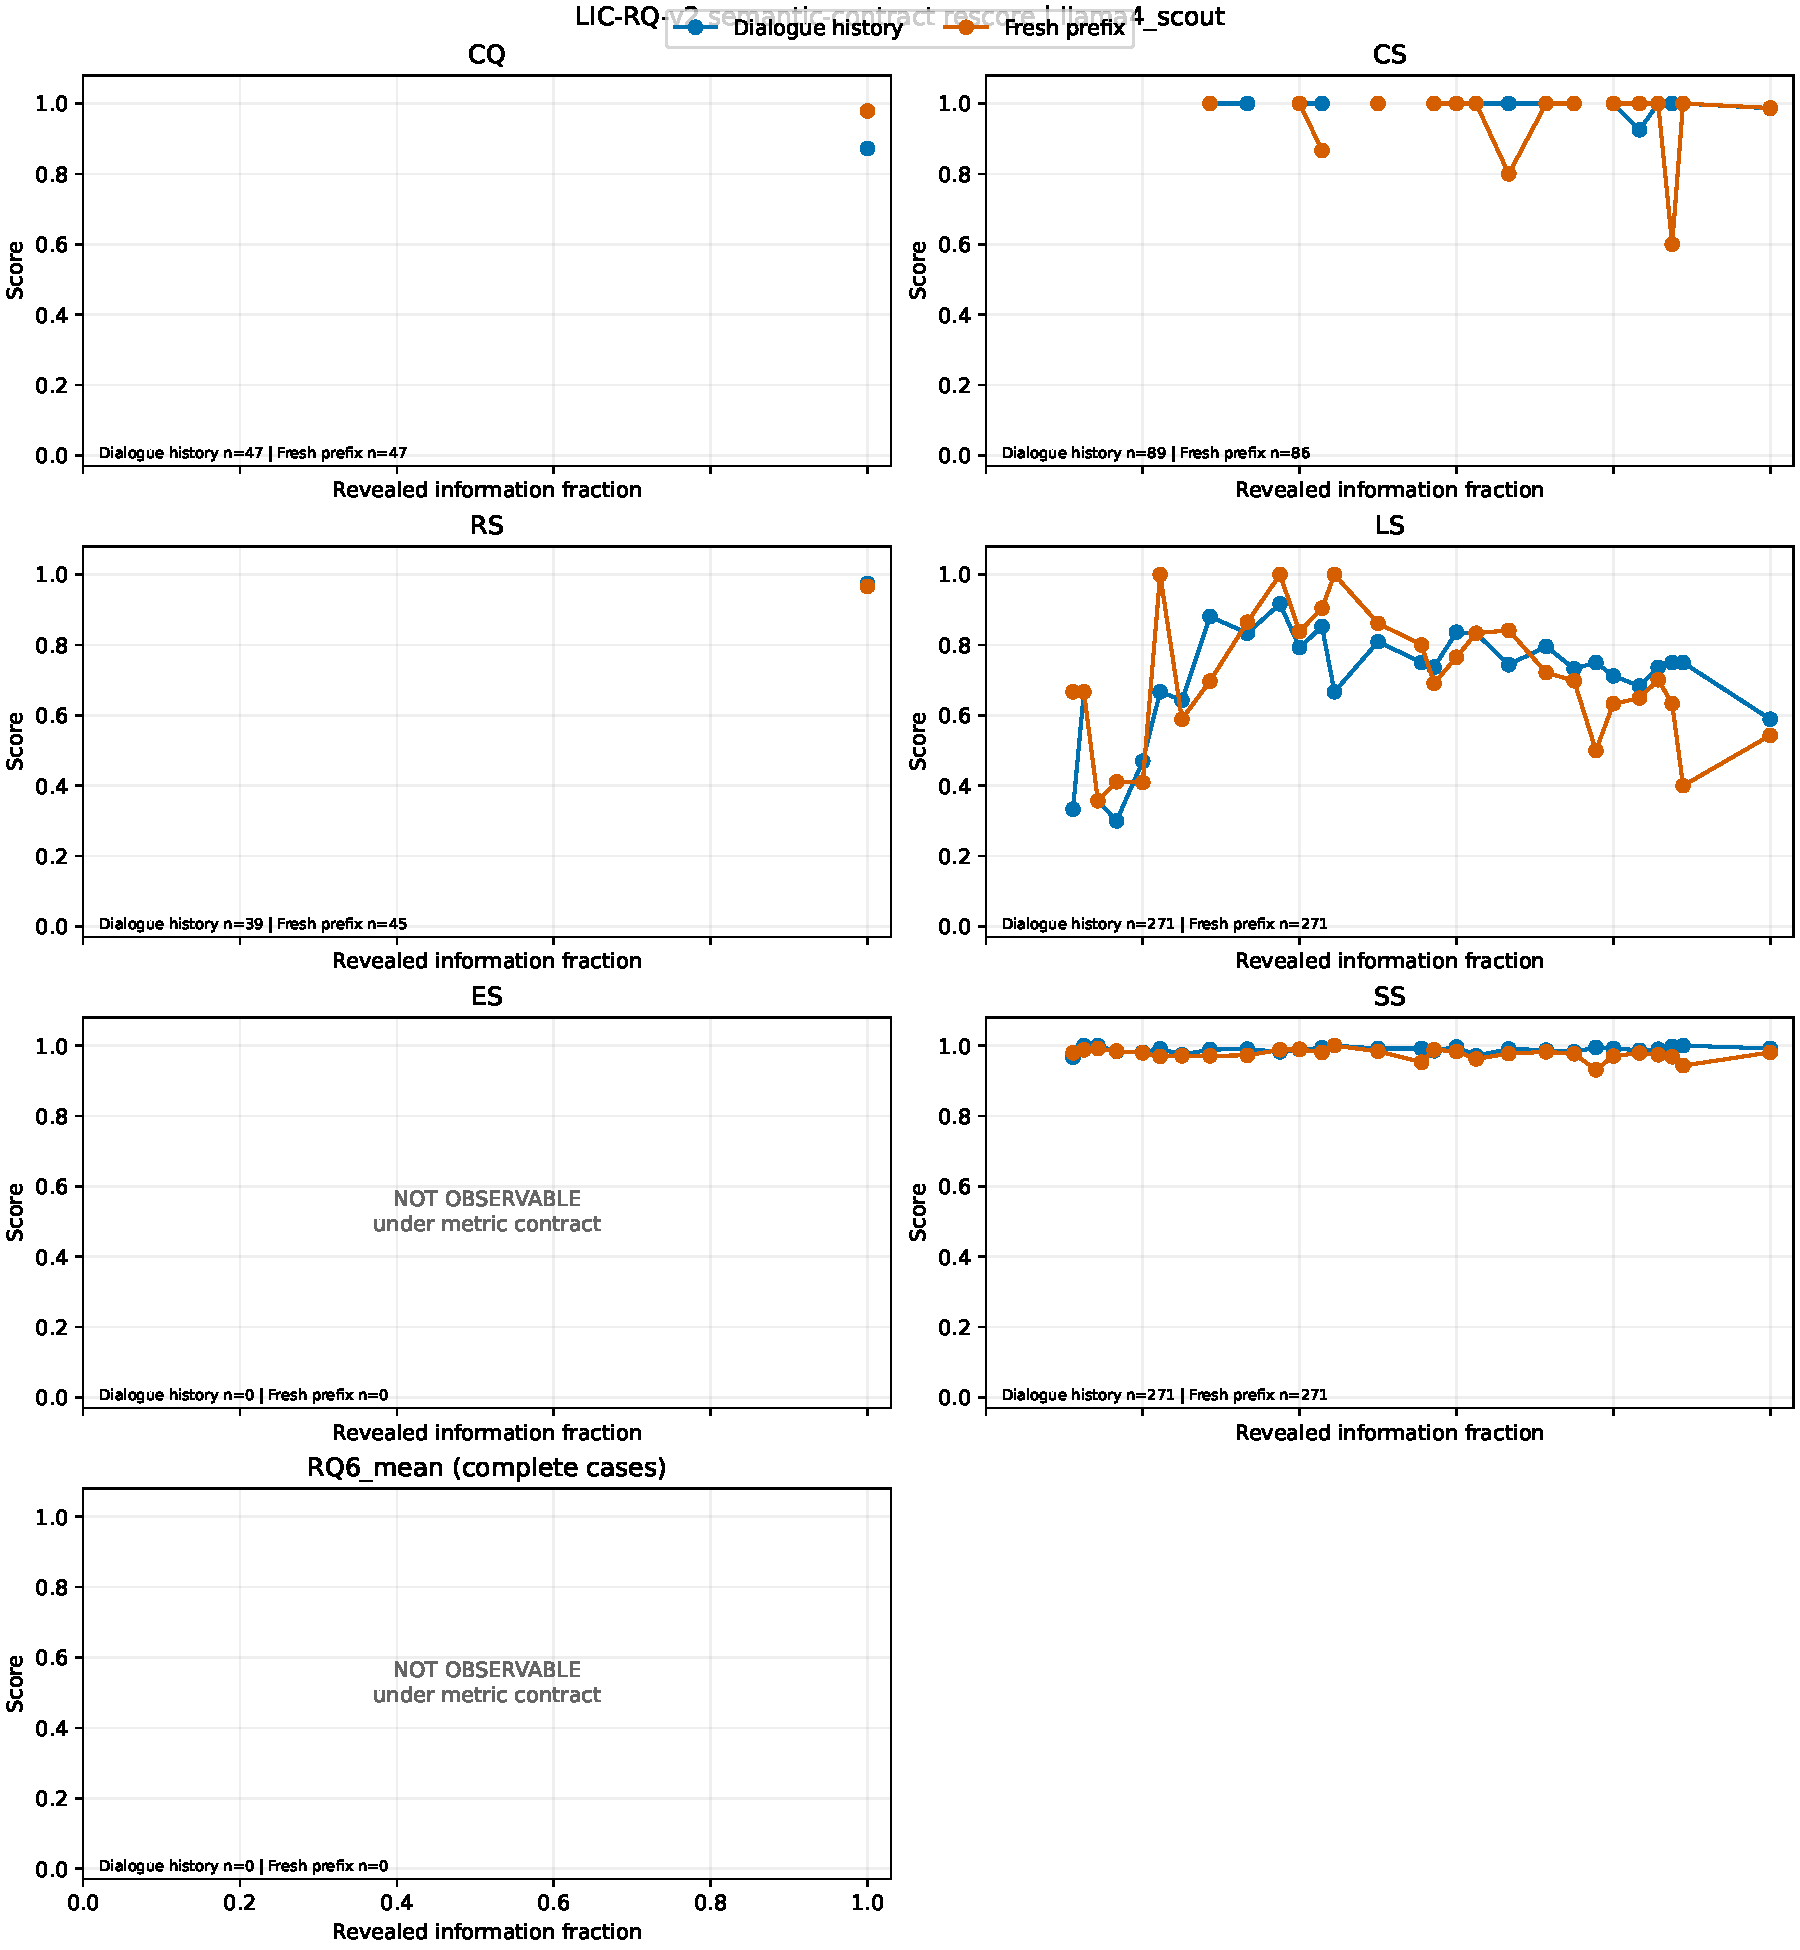
\includegraphics[width=0.85\linewidth]{supp_s1_metrics_llama4_scout.pdf}
\caption{Study 1, Llama-4 Scout.}\end{figure}
\begin{figure}[htbp]\centering
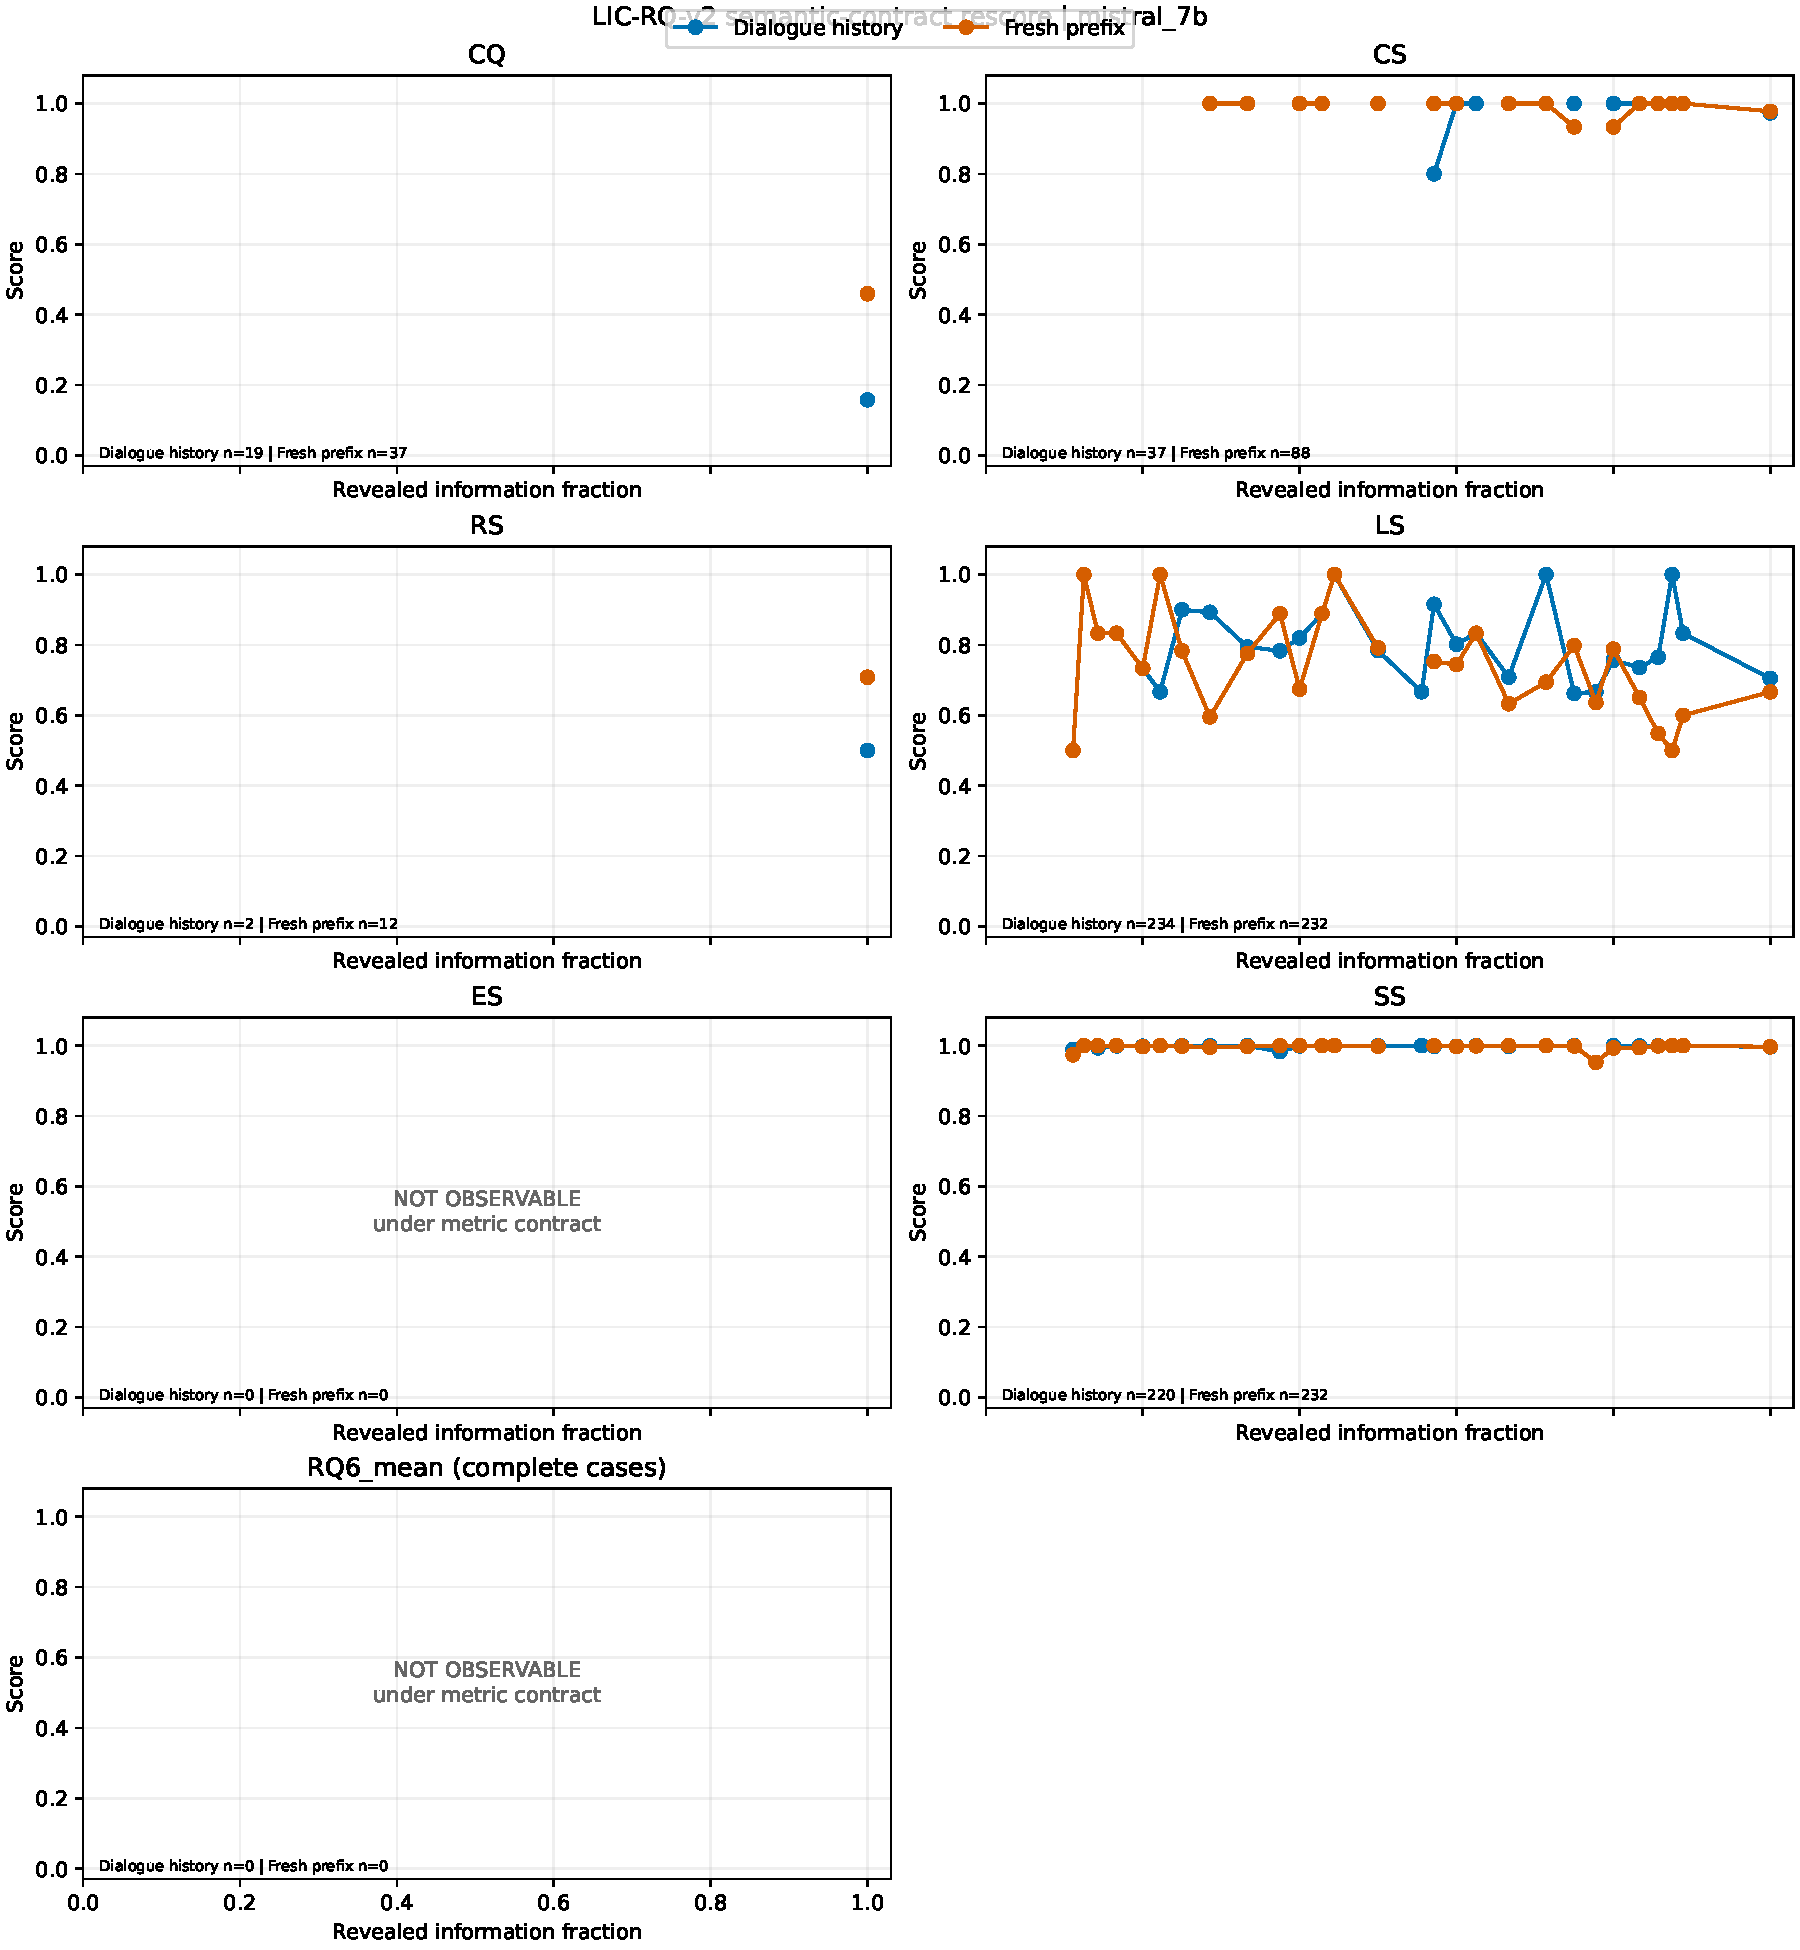
\includegraphics[width=0.85\linewidth]{supp_s1_metrics_mistral_7b.pdf}
\caption{Study 1, Mistral-7B.}\label{fig:s1mistral}\end{figure}

\subsection{Post-hoc stream replay}
Completed sessions were replayed as stream items with the regime switching
from fresh prefix to dialogue history, suddenly or gradually, over the same 48
tasks, with $W\in\{10,20,30\}$, five detectors and three assignment strategies.
Thresholds were set on 2,000 permutation nulls at family-wise $\alpha=0.05$ and
checked on 2,000 disjoint nulls. Table~\ref{tab:replay} gives the highest
detection rate per model and scenario. Over 180,000 replay rows, the historical
ADWIN never alarmed and the corrected ADWIN and CUSUM alarmed five times each,
with no early-warning candidate (Section~\ref{sec:adwin}).

\begin{table}[h]\centering\small
\caption{Study 1 replay at $W=20$ (post hoc): highest detection rate over the
validated cells.}
\label{tab:replay}
\begin{tabular}{llcl}\toprule
Model & Scenario & Max.\ detection & Metric / strategy\\\midrule
\inputtable{generated/table_replay.tex}
\bottomrule\end{tabular}\end{table}

\section{Study 2}

\subsection{Generator, ladder and mappings}
Each user turn realises one or more state events, may add distractor
sentences, and asks one question. Exact solvers keep the state and compute the
gold; the generator checks a solver round trip at every turn and that reworded
questions re-derive the same answer. Table~\ref{tab:ladder} gives the ladder, in
which exactly one axis changes per step; levels 13--14 are contingency levels
used only under the frozen ceiling rule. Table~\ref{tab:s2map} gives the frozen
mappings.

\begin{table}[h]\centering\small
\caption{Frozen difficulty ladder. Axes: query terms, events per turn,
distractor sentences and event complexity. $\dagger$: contingency levels.}
\label{tab:ladder}
\begin{tabular}{ccccc}\toprule
Level & Query terms & Events & Distractors & Complexity\\\midrule
\inputtable{generated/supp_ladder.tex}
\bottomrule\end{tabular}\end{table}

\begin{table}[h]\centering\small
\caption{Frozen difficulty mappings: ladder levels for the easy, medium and
hard regimes (E/M/H). A dash marks a domain excluded by the calibration rule.}
\label{tab:s2map}
\begin{tabular}{lcccc}\toprule
Model & Budget & Inventory & Laboratory & Milestones\\\midrule
\inputtable{generated/table_cdr_mappings.tex}
\bottomrule\end{tabular}\end{table}

\subsection{Difficulty calibration and model selection}
\label{sec:s2-calibration}
The frozen calibration rule fitted accuracy by isotonic regression and required
a one-sided Cochran--Armitage trend test with $p\le0.01$, adjacent-regime gaps of
at least 0.10 and an easy--hard gap of at least 0.25; a domain failing any
condition was excluded. A model was excluded if contract validity fell below
0.90 or any response was truncated. Over several frozen rounds, a coarse first
ladder was replaced by the one-axis-per-step ladder and a scheduling domain by
the milestone domain. Candidate models were replaced before any stream result
existed: Mistral-7B sat at the accuracy floor and truncated responses, the
gateway truncated a frontier model's outputs in one domain, and Gemma~4 31B
stayed at the ceiling even at the contingency levels and was replaced by Gemma
3 12B. Consistency and stability need diverse repeats. Llama-4 Scout produced
near-identical samples, and among the Llama variants only Llama-3 70B met the
frozen 0.80 diversity gate (Table~\ref{tab:kdiv}); a probe confirmed that it
accepts the full 100-turn history (37,139 prompt tokens) and recalls its oldest
message.

\begin{table}[h]\centering\small
\caption{Raw-text repeat diversity of Llama-family models on identical prompts.
Gate: diversity $\ge0.80$, contract validity $\ge0.90$, no truncation.}
\label{tab:kdiv}
\begin{tabular}{llccc}\toprule
Model (endpoint) & Prompts & Diversity & Validity & Truncated\\\midrule
\inputtable{generated/supp_kdiv.tex}
\bottomrule\end{tabular}\end{table}

\subsection{Deviations, acquisition and staged analysis}
Two deviations for Llama-3 70B were recorded after the relevant gate results.
One of its 1,440 calibration responses reached the 2,048-token ceiling, in a
domain excluded for this model on accuracy grounds, and the any-truncation rule
was overridden for this model only; Mistral-7B had been excluded under the same
rule with five truncations. Its technical pilot also had two truncated
non-primary responses, both repetition loops, and the pilot's zero-truncation
gate was overridden. In its place a truncation policy was frozen for all models
before the main run: a truncated reply is kept verbatim and scored as missing,
a truncated primary enters later history as a placeholder, and a sensitivity
analysis rescores truncated cells as incorrect.

The budget paused the main run twice. At the second pause, 25,039 of 54,000
calls had been made; all 90 dialogue-history primary chains were complete
except one Llama-3 70B turn-100 primary. The analysis protocol was frozen
before any main-run metric was computed. Stage A analysed every fully acquired
model--metric pair; Stage B, covering the remaining repeat-based samples and
controls for Llama-3 70B and Gemma 3 12B, was committed before any Stage A
result was seen. Its control arms (3,000 calls per model) were later completed
under a separately frozen protocol (test H-C1 in the article); its repeat-based
samples were not. At Stage A, Llama-3 70B had two truncated primaries, and
scoring them as incorrect changed no result.

\begin{figure}[htbp]\centering
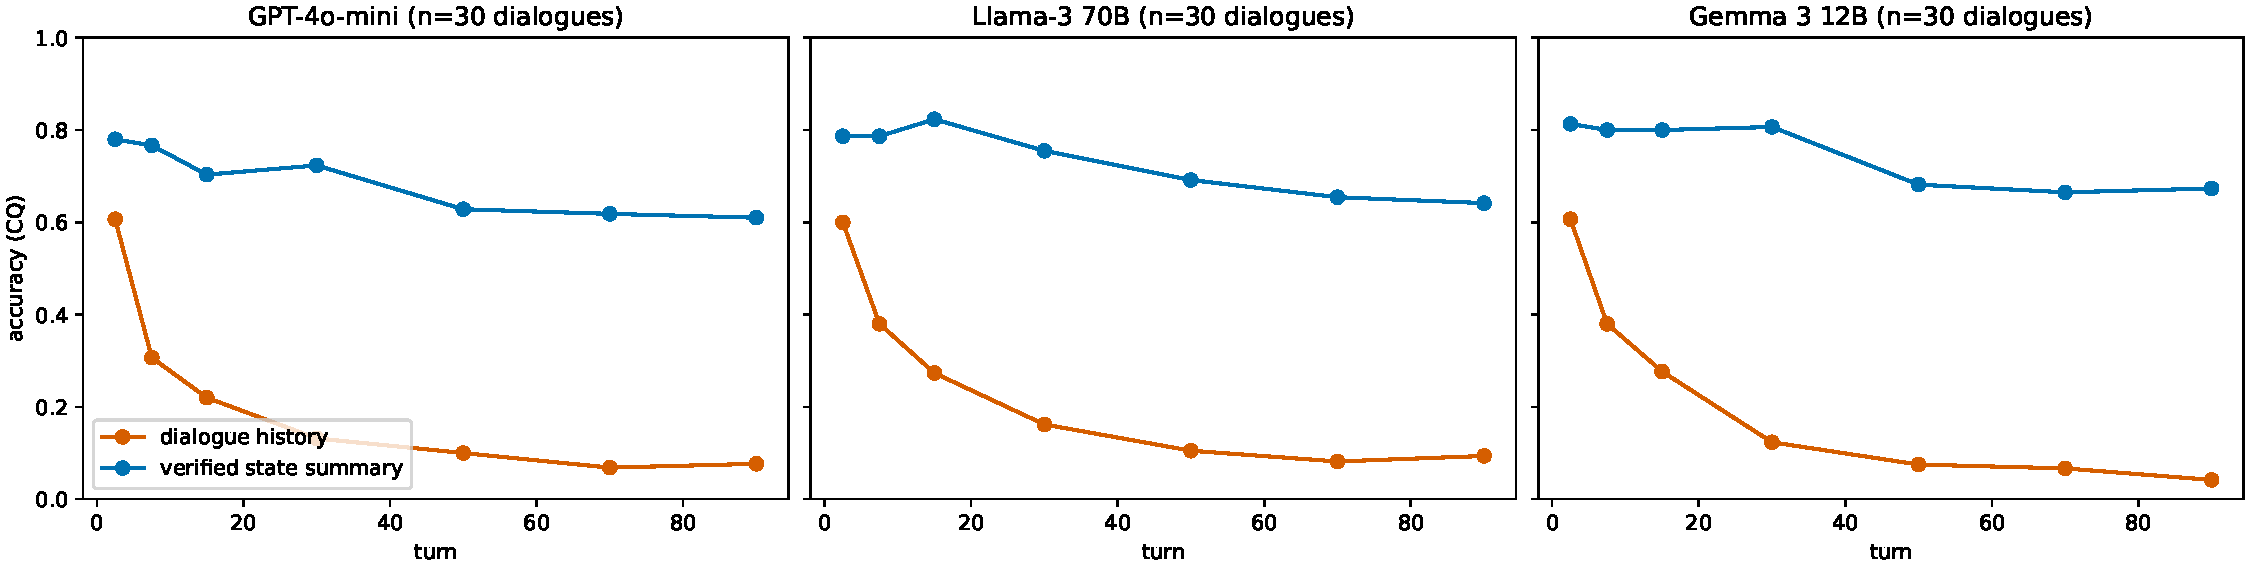
\includegraphics[width=0.8\linewidth]{supp_s2_control_completion.pdf}
\caption{Dialogue-history and verified-state-summary accuracy over turns for
the three Study 2 models.}
\label{fig:s2controlcompletion}
\end{figure}

\subsection{Frozen change-point contrasts}
The confirmatory Stage A contrasts compare the 20 turns after each change point
with the 20 turns before it (Table~\ref{tab:h1a}). Because the dialogue arm
collapses from turn 1, even in stationary dialogues, they mix task drift with
the background collapse and are not interpreted as task-drift effects. The
dialogue-minus-control contrast H1b, available for GPT-4o-mini only, was
uninformative under this floor (mean differences 0.03--0.23, Holm $p=1.0$).

\begin{longtable}{llcccc}
\caption{Stage A H1a (confirmatory): post-minus-pre window means in the
dialogue arm, pooled over models with model-stratified sign flips. CS, RS and
SS are GPT-4o-mini only.}
\label{tab:h1a}\\
\toprule Transition & Metric & Mean $\Delta$ & Dialogues & $p$ & $p_{\text{Holm}}$\\\midrule
\endfirsthead
\toprule Transition & Metric & Mean $\Delta$ & Dialogues & $p$ & $p_{\text{Holm}}$\\\midrule
\endhead
\inputtable{generated/supp_h1a.tex}
\bottomrule
\end{longtable}

\subsection{Detector strategies and dialogue-arm monitoring}
Table~\ref{tab:strategies} gives the three detector assignments and
Table~\ref{tab:stagea} the dialogue-arm detection rates; n/c means that no grid
value met the null false-alarm target, because the stationary dialogues also
decline.

\begin{table}[h]\centering\small
\caption{Detector assignment strategies. All monitor a decrease of the window
mean; CQ is additionally monitored on its raw binary stream by DDM.}
\label{tab:strategies}
\begin{tabular}{lcccccc}\toprule
Strategy & CQ & CS & RS & LS & ES & SS\\\midrule
Distribution-based & CUSUM & CUSUM & CUSUM & CUSUM & CUSUM & CUSUM\\
Proposal mapping & CUSUM & ADWIN & DDM & PH & EWMA & ADWIN\\
ADWIN everywhere & ADWIN & ADWIN & ADWIN & ADWIN & ADWIN & ADWIN\\
\bottomrule\end{tabular}\end{table}

\begin{table}[h]\centering\small
\caption{Stage A dialogue-arm detection rate within 33 turns of the first
change, with thresholds calibrated on the 36 pooled stationary dialogues.}
\label{tab:stagea}
\begin{tabular}{llcccccc}\toprule
$W$ & Strategy & CQ & CS & RS & LS & ES & SS\\\midrule
\inputtable{generated/supp_stagea_monitoring.tex}
\bottomrule\end{tabular}\end{table}

\subsection{Control-arm monitoring}
\label{sec:control-monitoring}
The rules were developed exploratorily on the GPT-4o-mini control arm
(Tables~\ref{tab:ctrlscreen} and~\ref{tab:early}) and then applied unchanged to
Llama-3 70B and Gemma 3 12B as a frozen validation (Table~\ref{tab:monitorvalidation},
Figure~\ref{fig:valagg}). On GPT-4o-mini, CQ CUSUM detected \ctrlScreenDetect{}
drift dialogues within 33 turns at $W=20$, and the baseline threshold rule
flagged accuracy in \earlyCqSignal{} drift but also \earlyCqNull{} stationary
dialogues; LS signalled in \earlyLsSignal{} drift dialogues, \earlyLsBefore{} of
them before accuracy, but also in \earlyLsNull{} stationary ones. Neither
validation model passed the single-stream screen, and the apparent LS leads did
not separate from alarms in stationary dialogues.

\begin{table}[h]\centering\small
\caption{GPT-4o-mini control arm (exploratory): per-dialogue detection rate
within 33 turns, with the leave-one-out false-alarm rate in parentheses, on 18
drift and 12 stationary dialogues.}
\label{tab:ctrlscreen}
\begin{tabular}{llccc}\toprule
$W$ & Strategy & CQ & LS & ES\\\midrule
\inputtable{generated/supp_control_screen.tex}
\bottomrule\end{tabular}\end{table}

\begin{table}[h]\centering\small
\caption{Per-dialogue threshold rule on GPT-4o-mini (exploratory). Baseline
turns 1--30; a signal is a window mean below $\mu_0-2\sigma_0/\sqrt{W}$ on three
consecutive turns. LS and ES timing relative to CQ: before/same/after.}
\label{tab:early}
\begin{tabular}{ccccccc}\toprule
$W$ & CQ signalled & CQ null & LS signalled & LS b/s/a & LS null & ES b/s/a\\\midrule
\inputtable{generated/supp_early_signal.tex}
\bottomrule\end{tabular}\end{table}

\begin{table}[h]\centering\small
\caption{Frozen monitoring validation at $W=20$. Null counts are alarms among
12 stationary dialogues for the LS rule and among two stationary scenario
aggregates for the six-dialogue CQ CUSUM.}
\label{tab:monitorvalidation}
\begin{tabular}{lcccccc}\toprule
Model & CUSUM detect & Delay & LS signal & LS null & Agg.\ detect & Agg.\ null\\\midrule
Llama-3 70B & \valLlamaDetect{} & \valLlamaDelay{} & \valLlamaLsSignal{} &
\valLlamaLsNull{} & \valLlamaAggDetect{} & \valLlamaAggNull{}\\
Gemma 3 12B & \valGemmaDetect{} & \valGemmaDelay{} & \valGemmaLsSignal{} &
\valGemmaLsNull{} & \valGemmaAggDetect{} & \valGemmaAggNull{}\\
\bottomrule\end{tabular}\end{table}

\begin{figure}[htbp]\centering
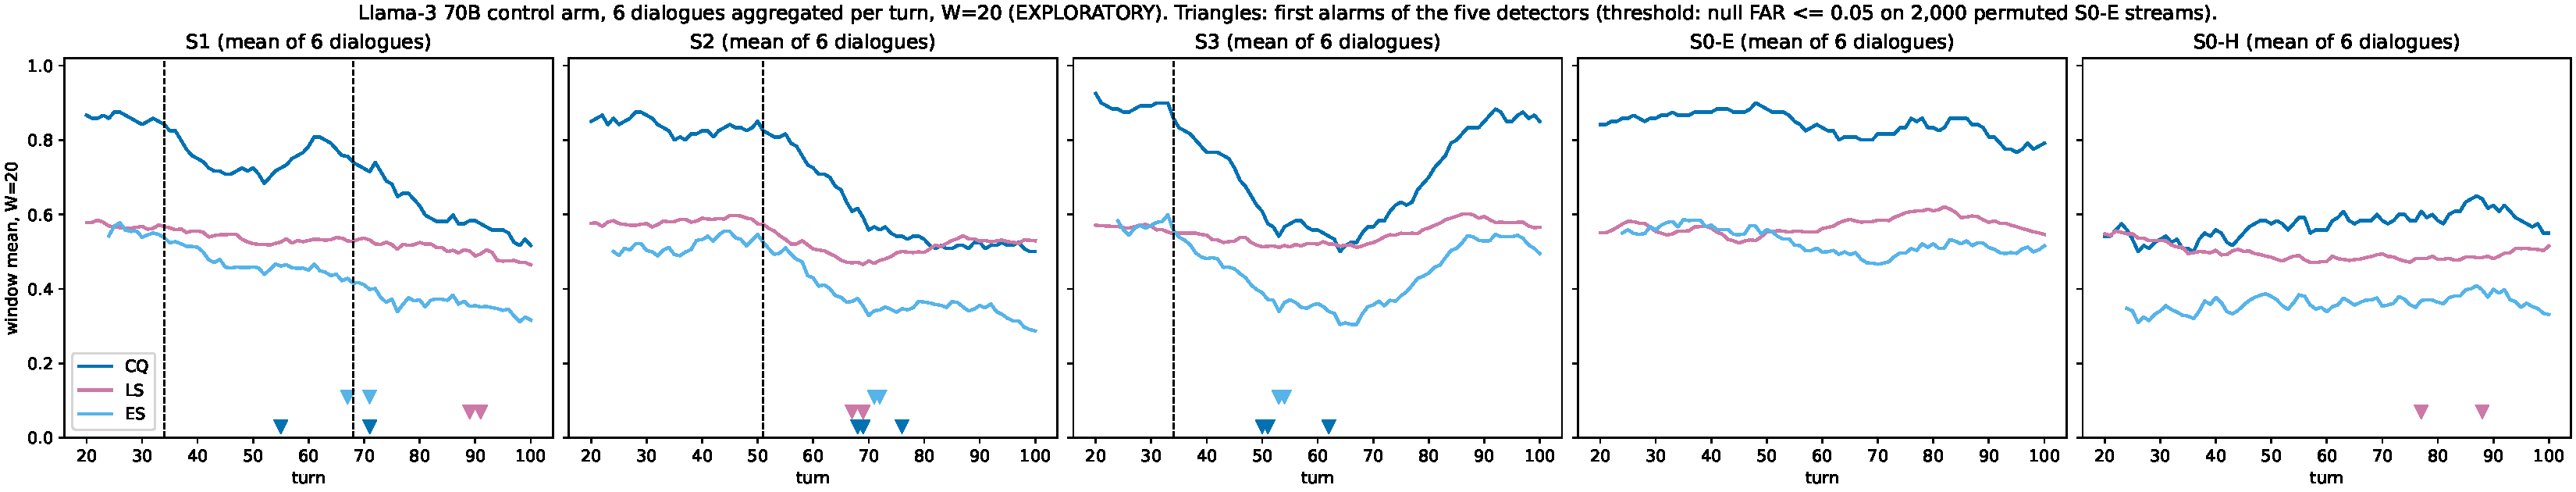
\includegraphics[width=\linewidth]{supp_s2_validation_llama_agg.pdf}\\[4pt]
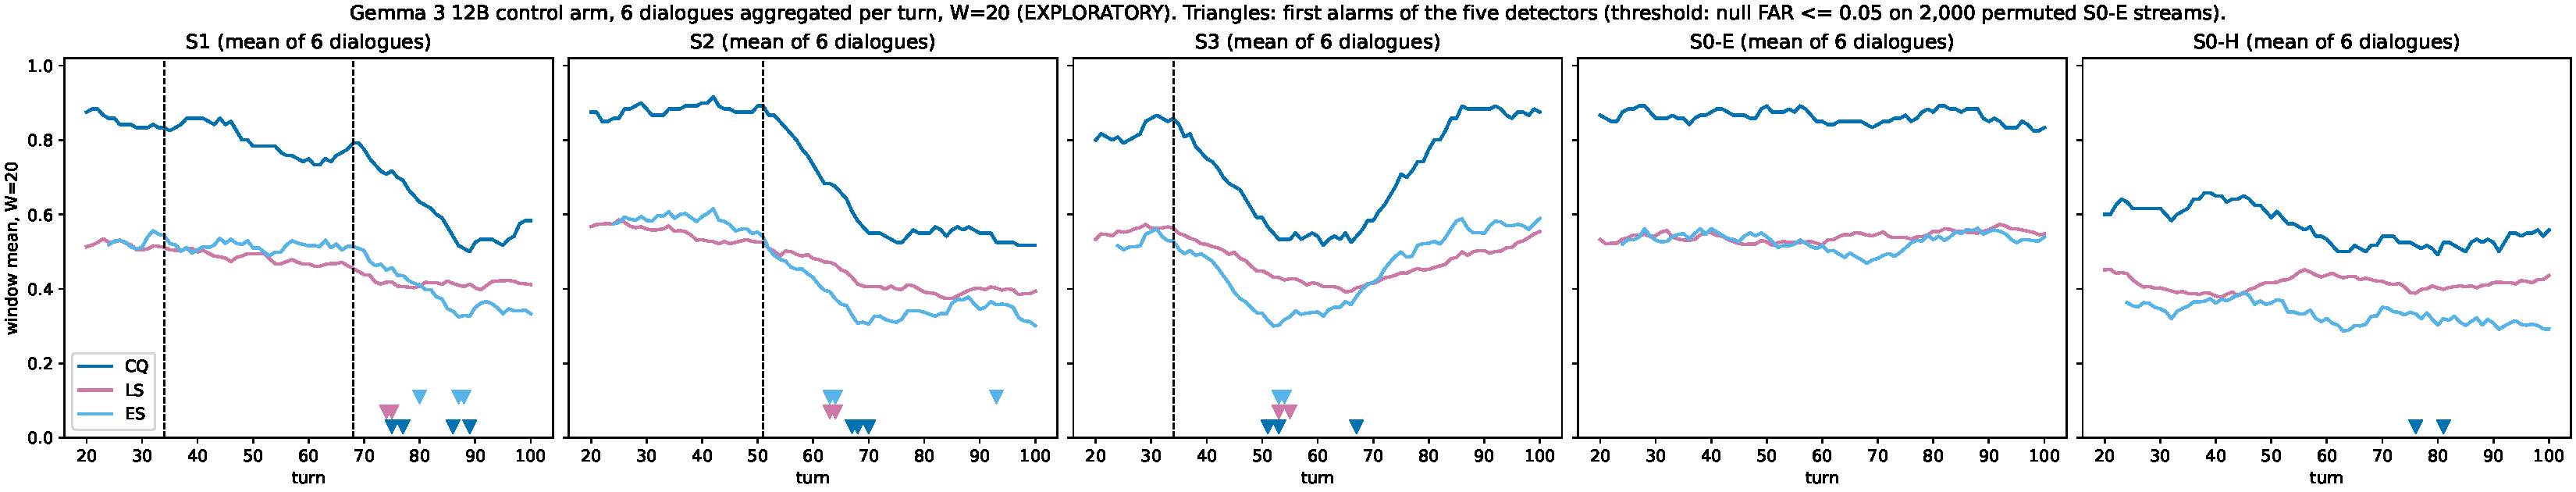
\includegraphics[width=\linewidth]{supp_s2_validation_gemma_agg.pdf}
\caption{Six-dialogue aggregate monitoring at $W=20$ in the frozen validation:
Llama-3 70B (top) and Gemma 3 12B (bottom).}\label{fig:valagg}\end{figure}

\subsection{Per-model trajectories (Stage A)}
\begin{figure}[htbp]\centering
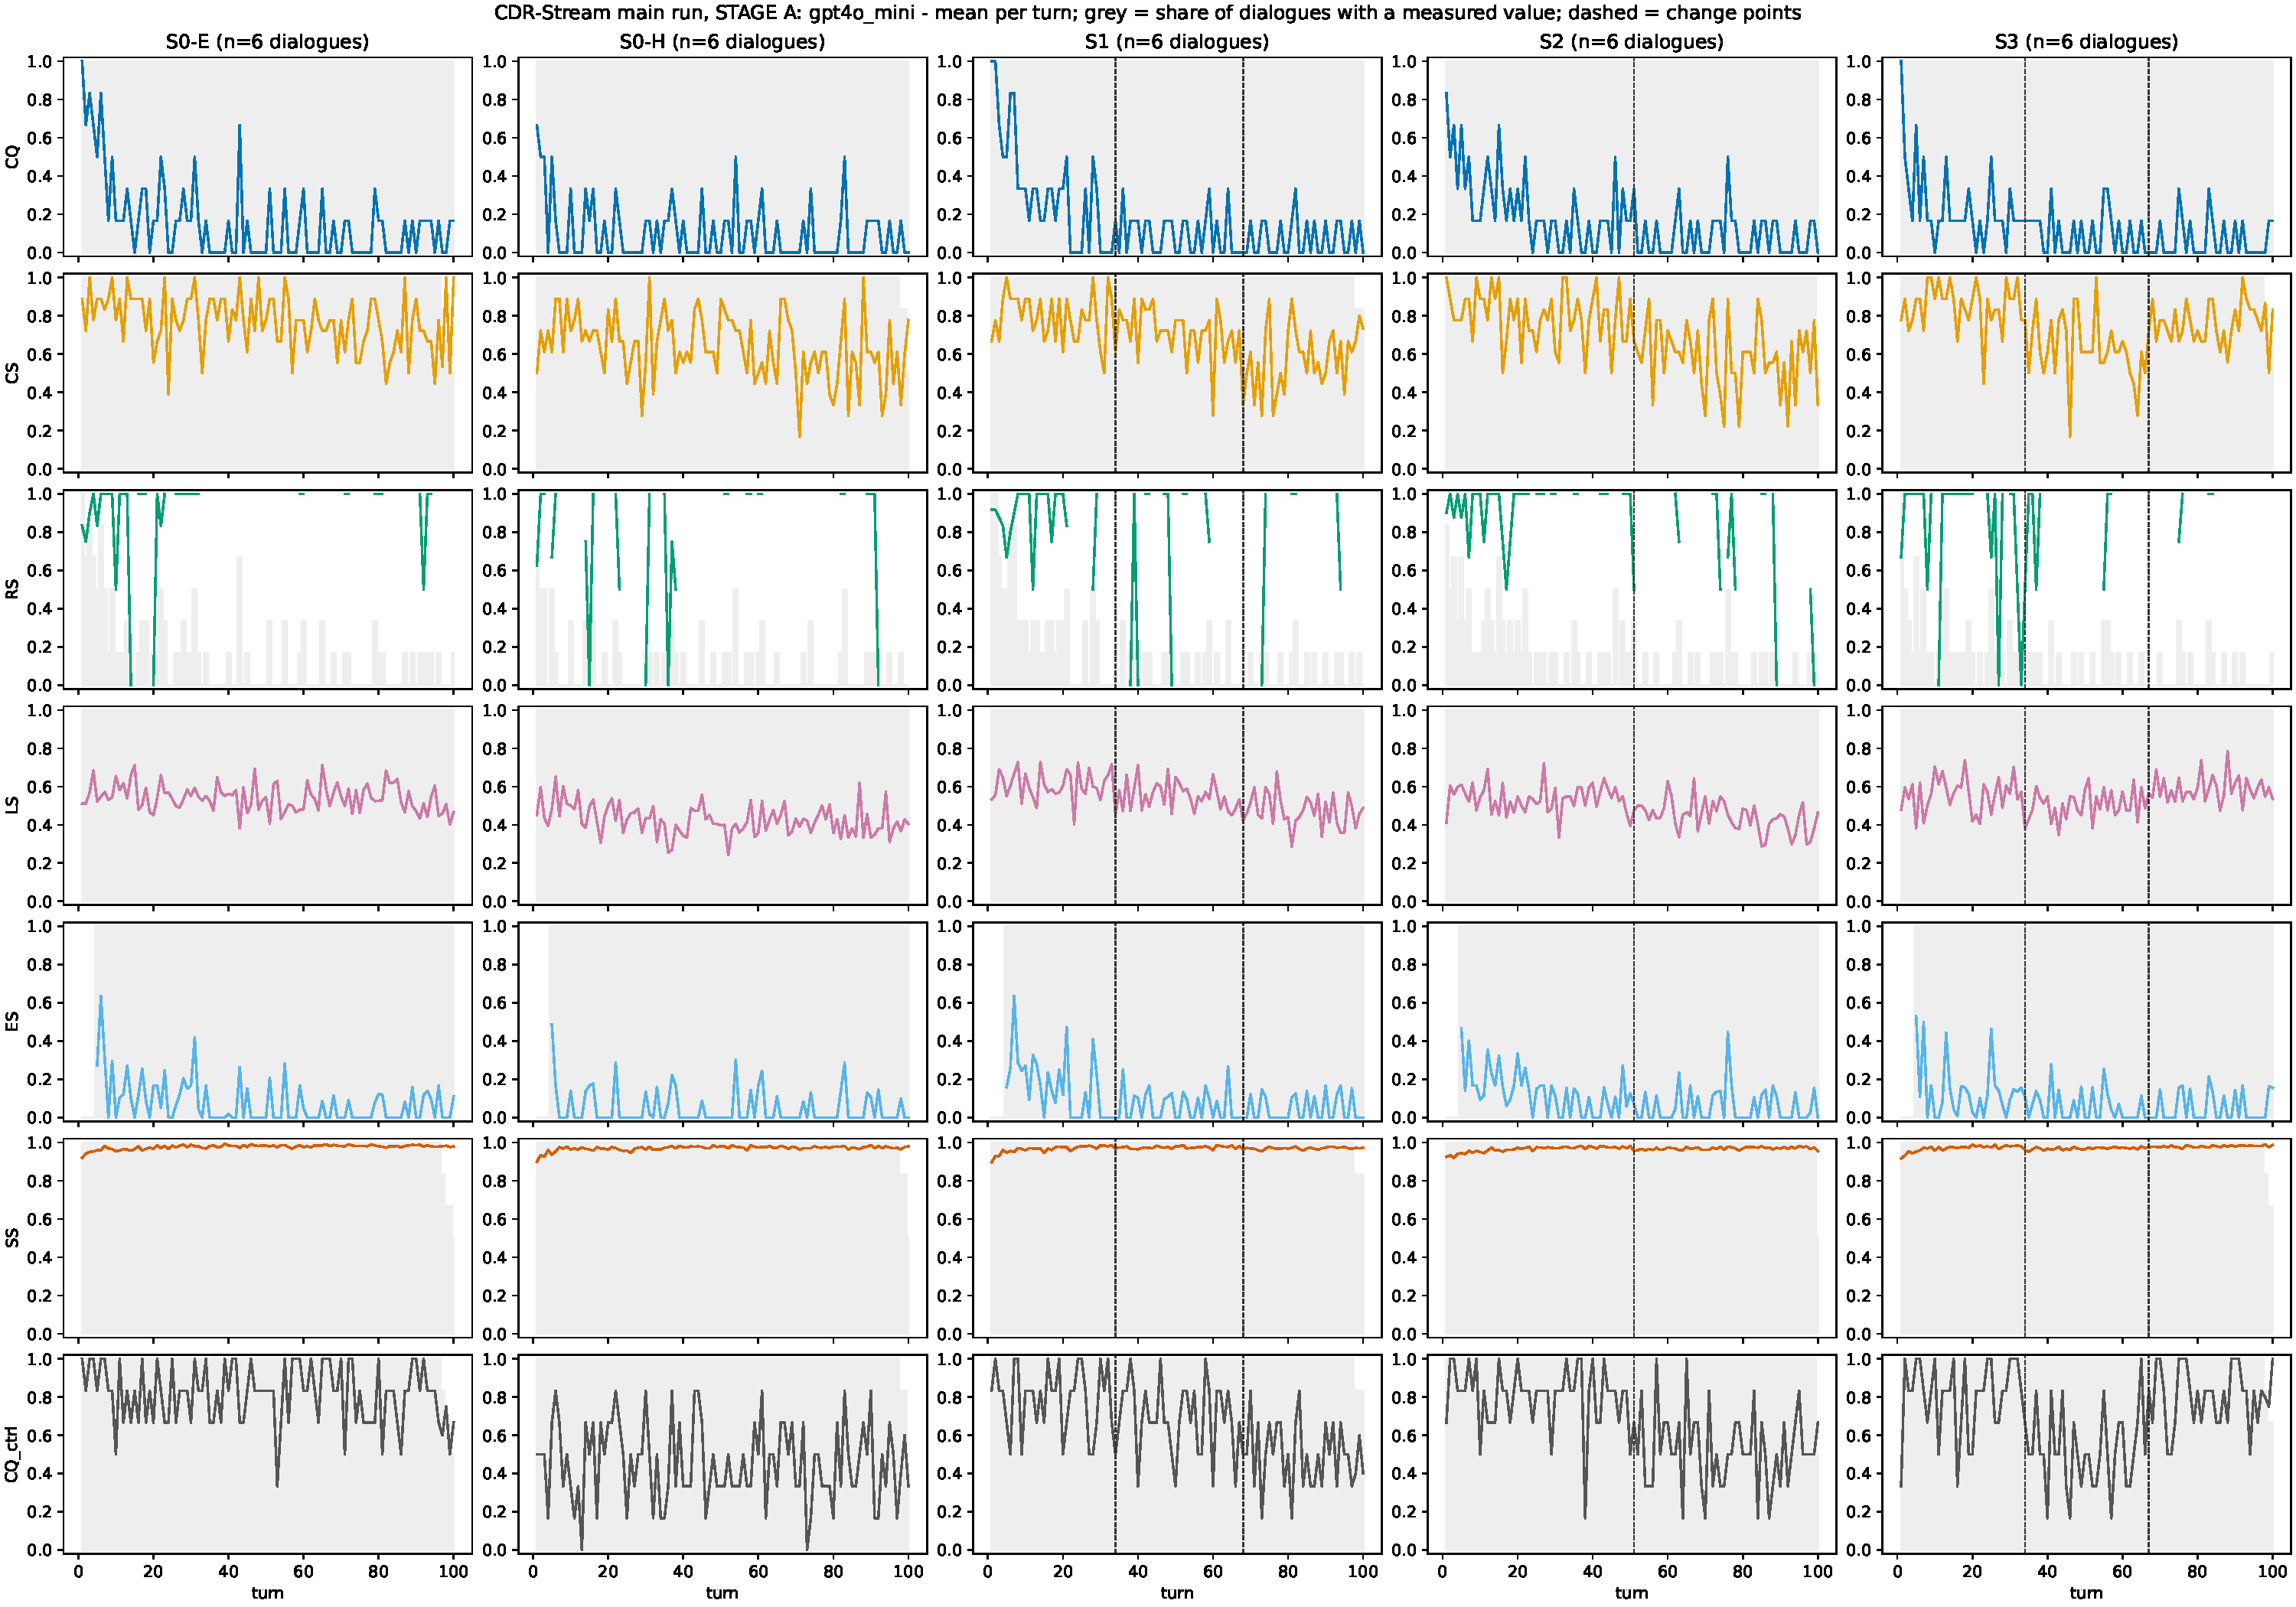
\includegraphics[width=0.85\linewidth]{supp_s2_metrics_gpt4o_mini.pdf}
\caption{Study 2, GPT-4o-mini: six dimensions and the control CQ by
scenario.}\end{figure}
\begin{figure}[htbp]\centering
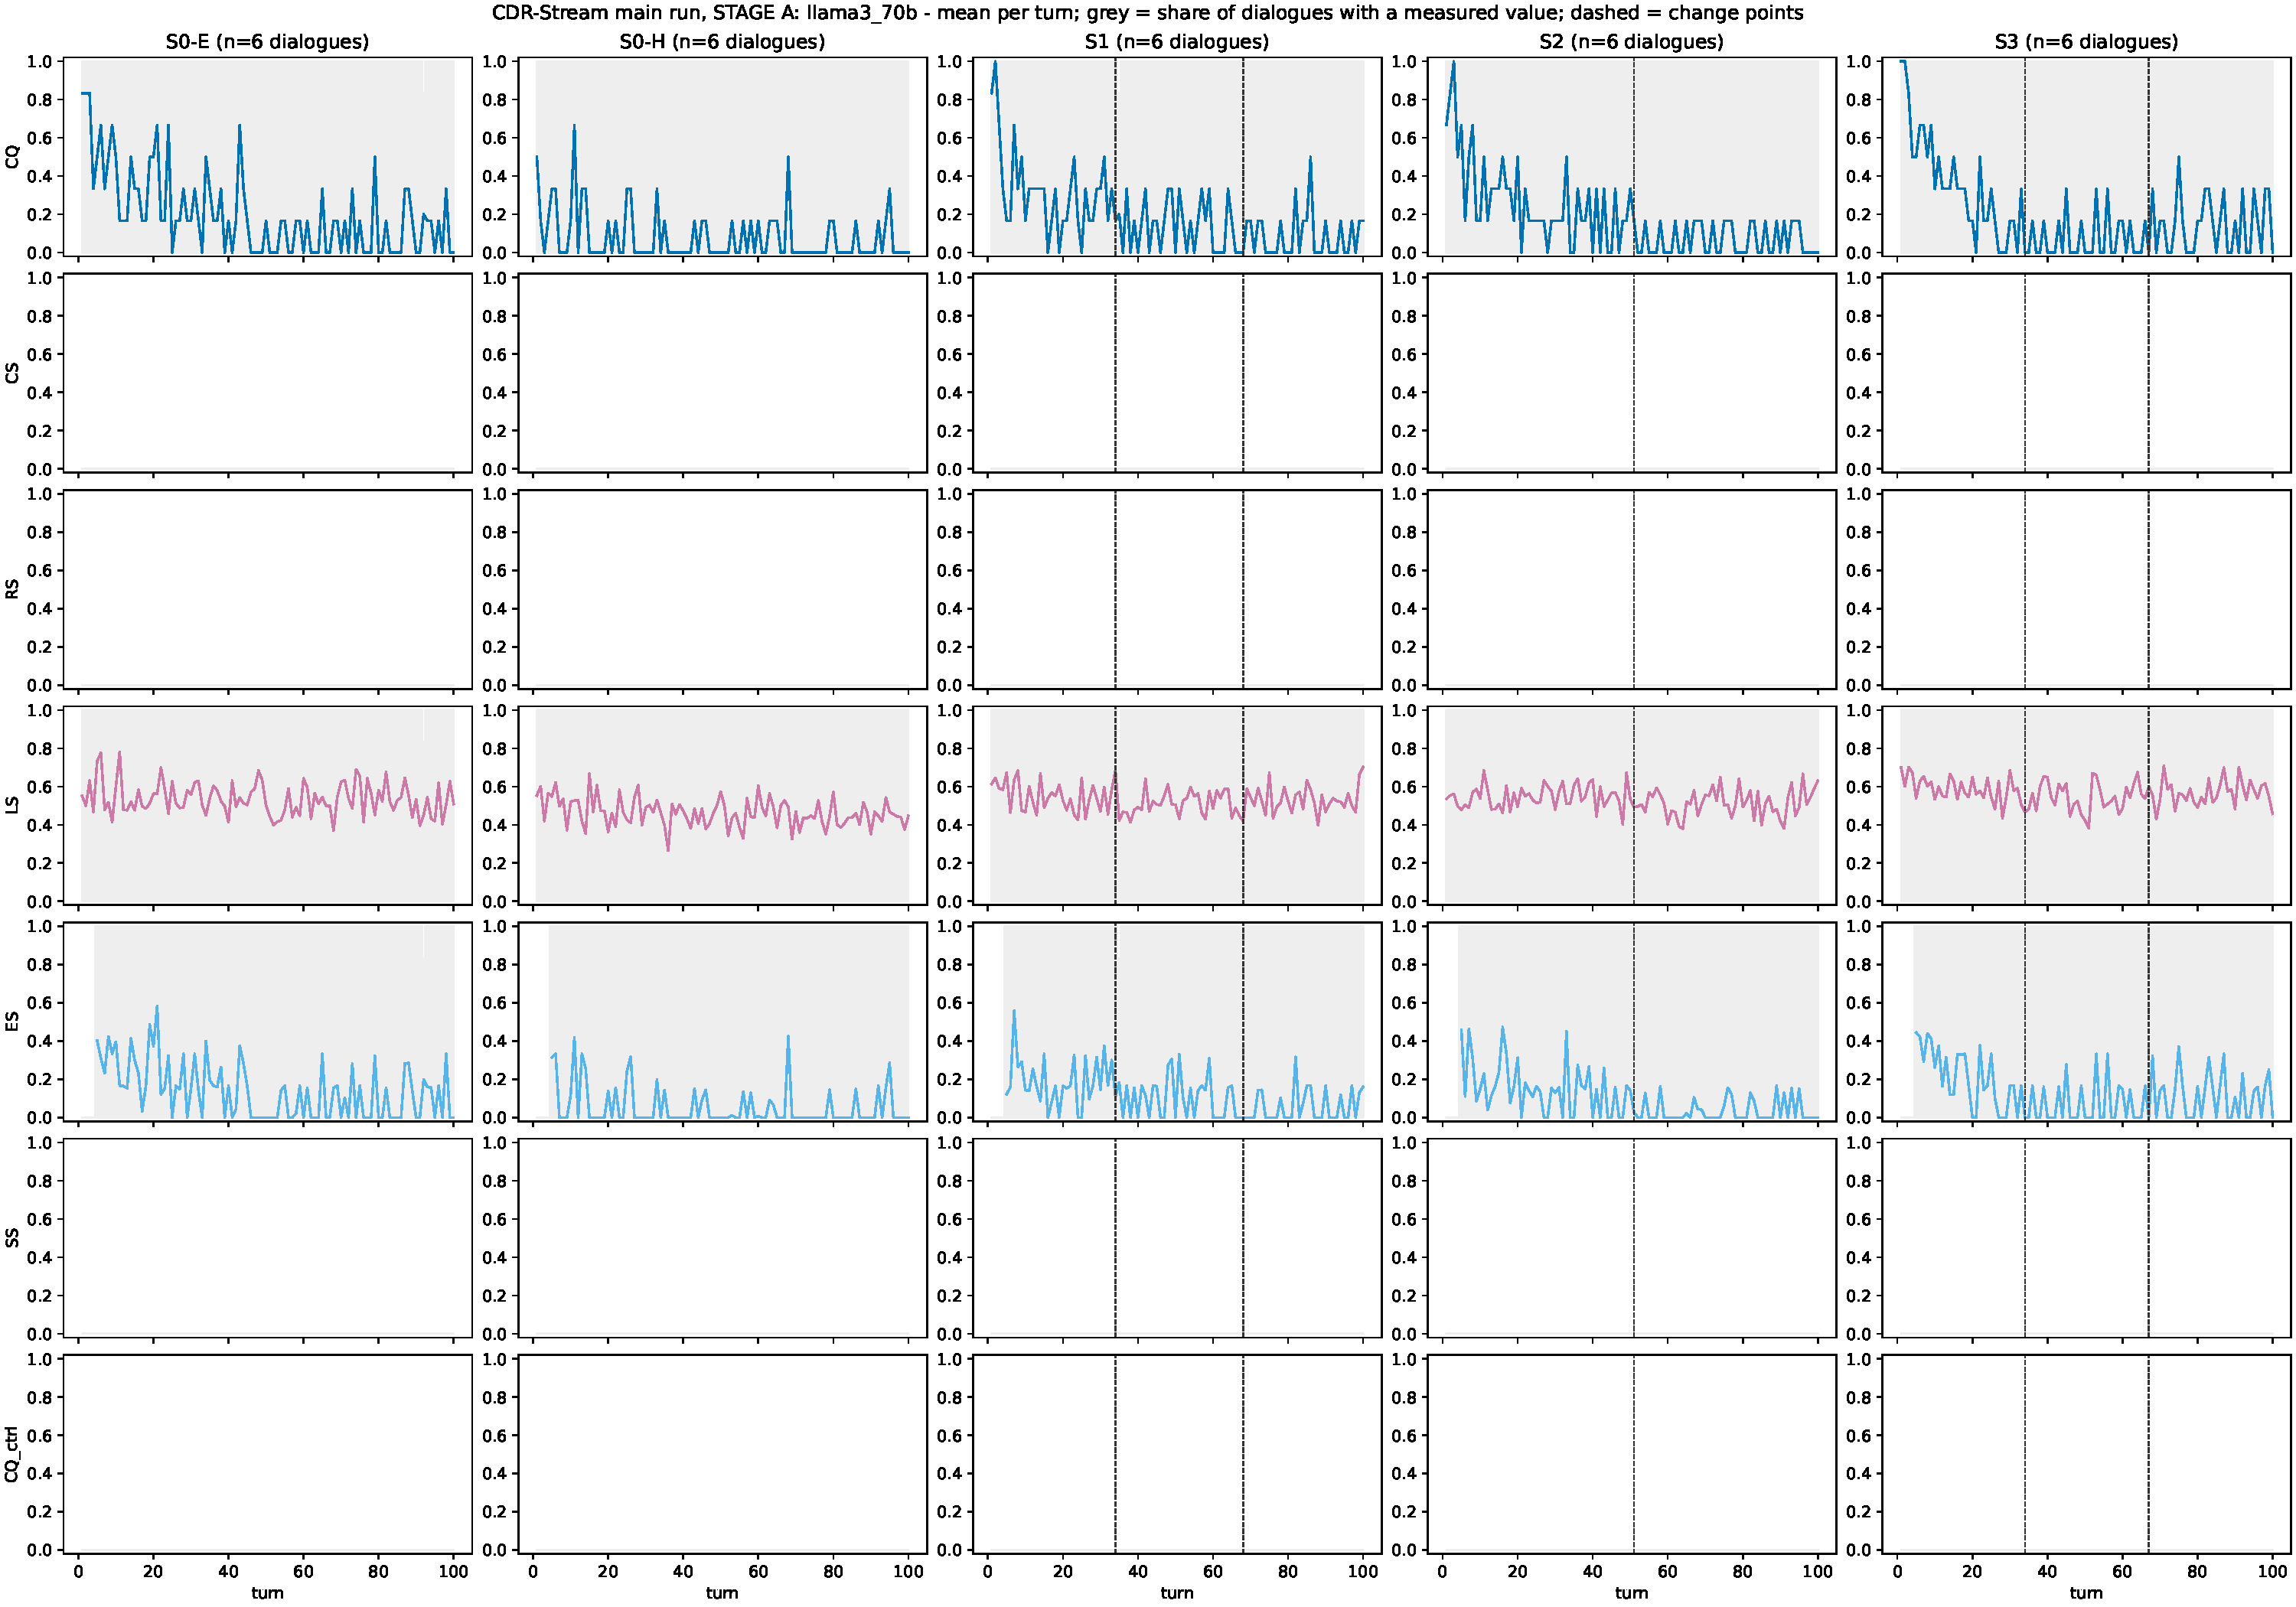
\includegraphics[width=0.85\linewidth]{supp_s2_metrics_llama3_70b.pdf}
\caption{Study 2 dialogue-arm metrics, Llama-3 70B. Repeat-based sampling was
not completed, so the CS, RS and SS panels are empty by design, not zero.}
\end{figure}
\begin{figure}[htbp]\centering
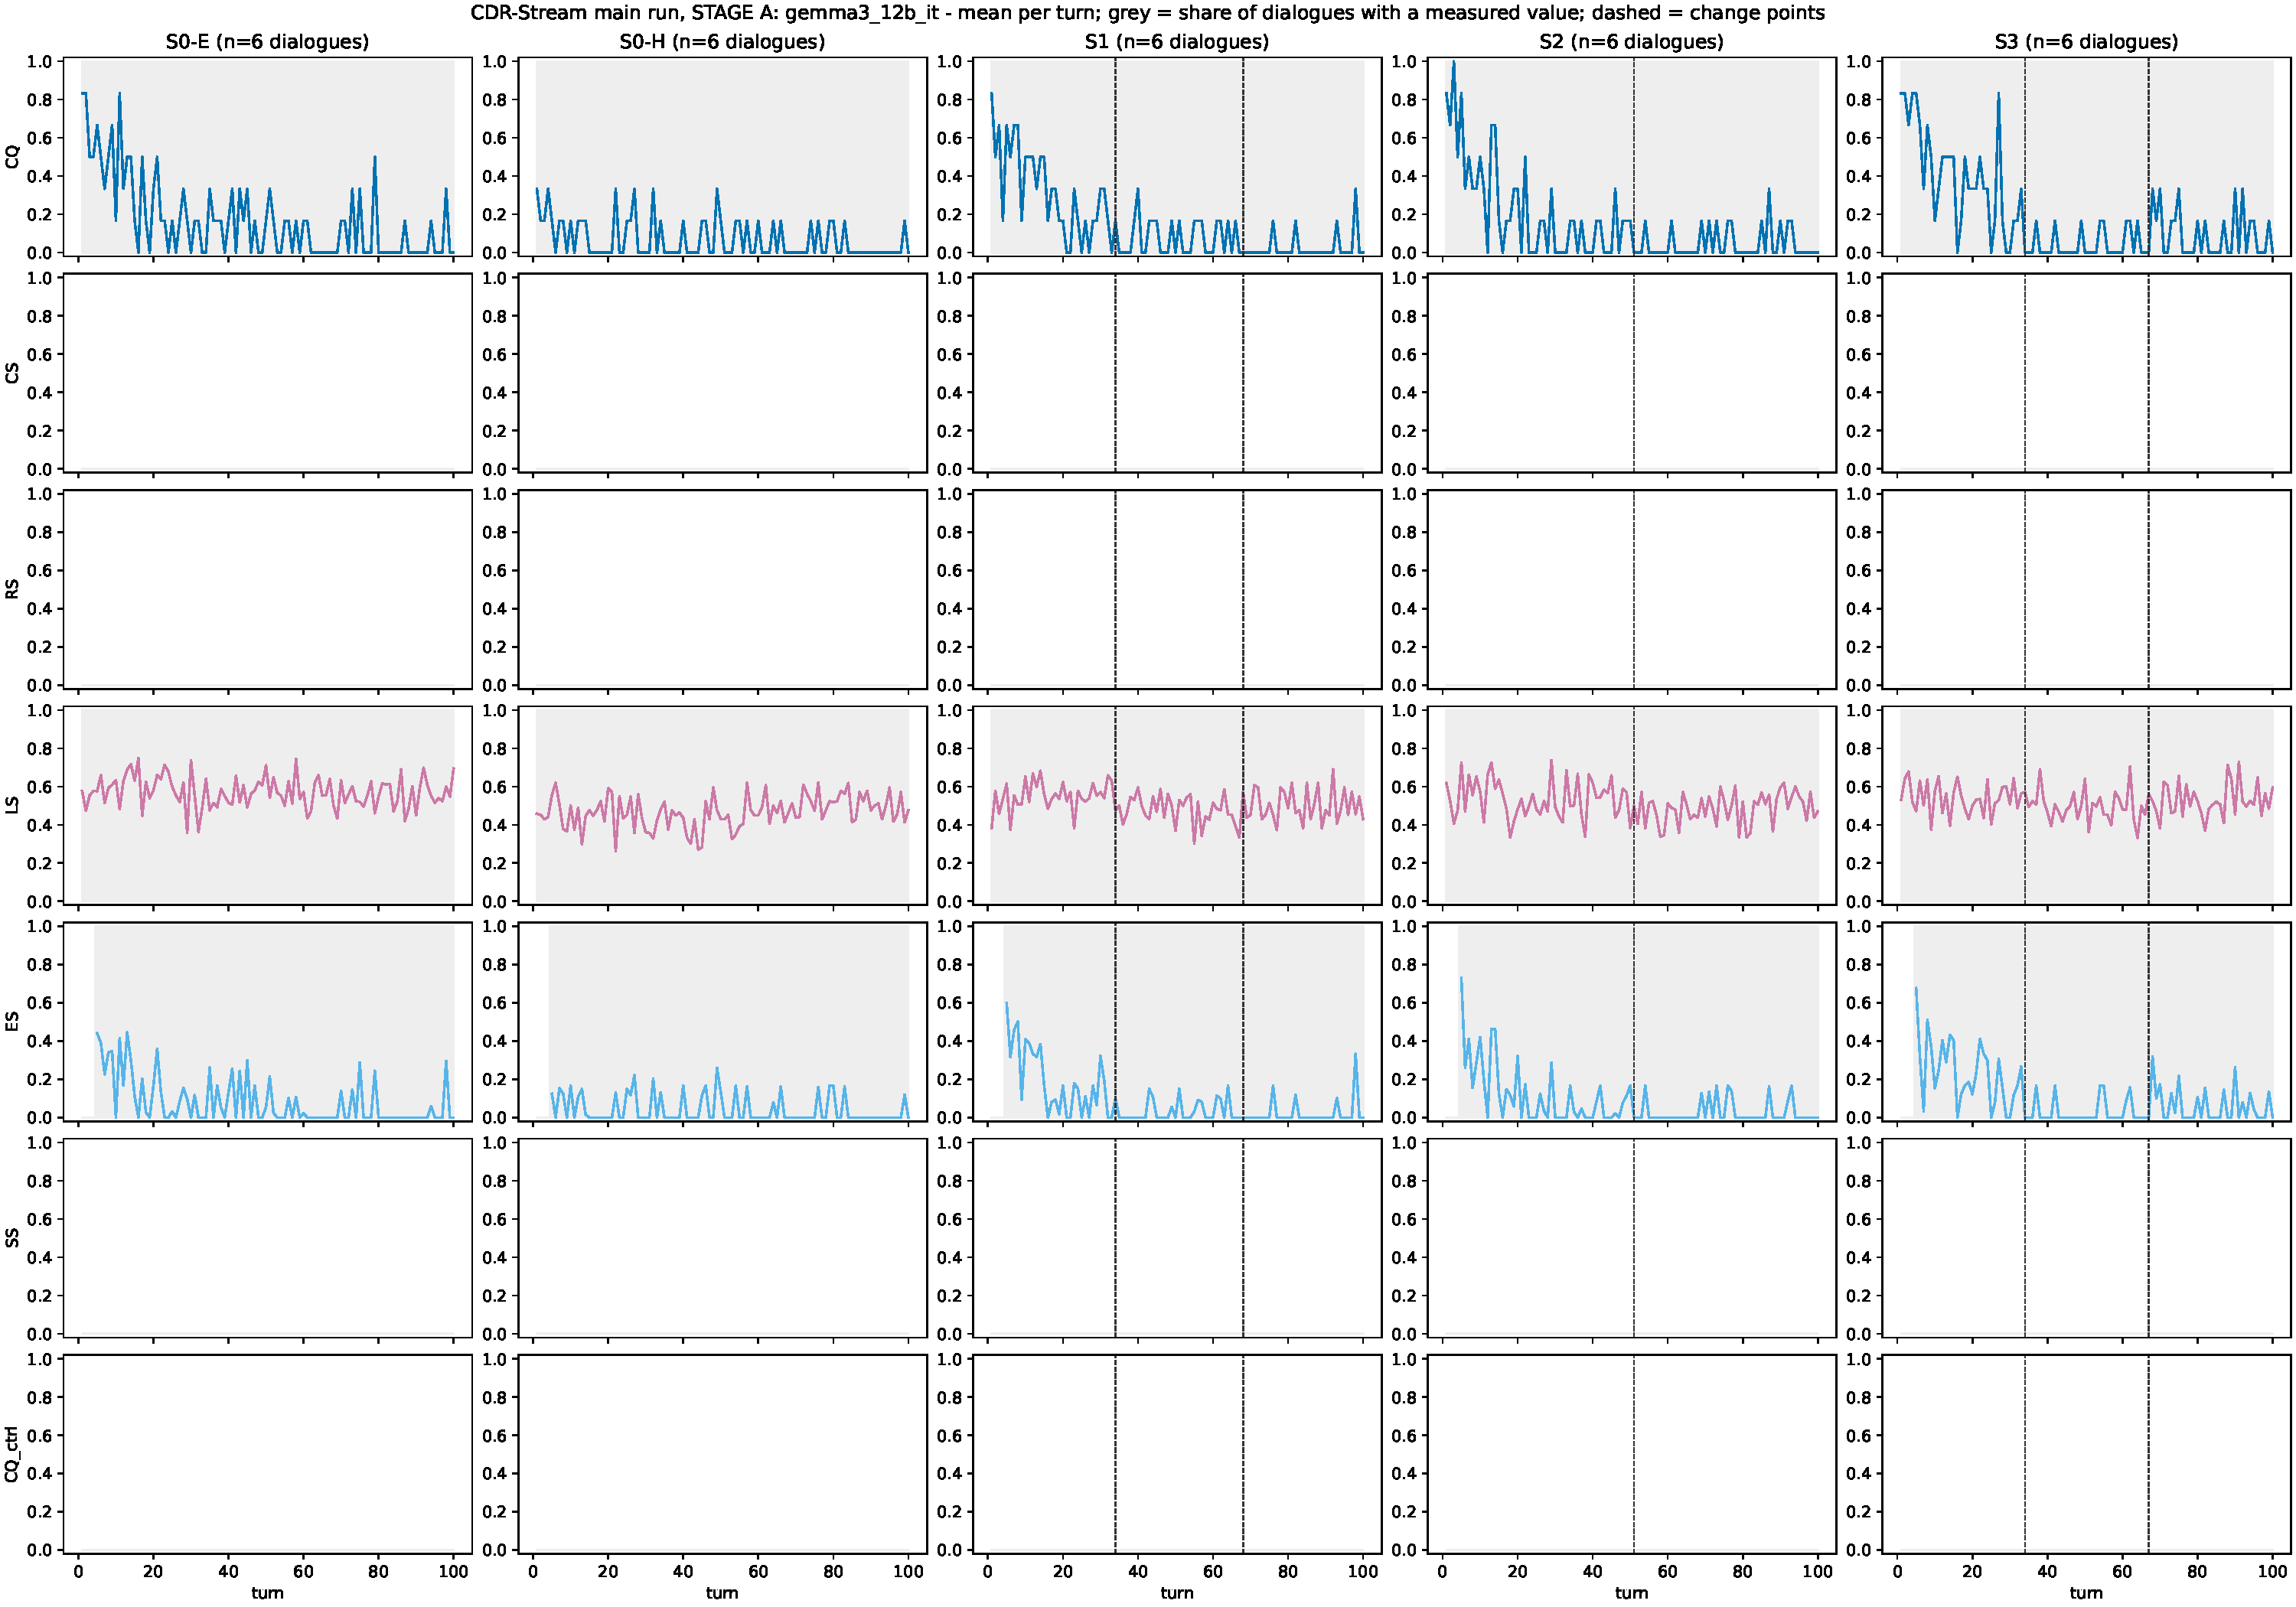
\includegraphics[width=0.85\linewidth]{supp_s2_metrics_gemma3_12b_it.pdf}
\caption{Study 2 dialogue-arm metrics, Gemma 3 12B. Repeat-based sampling was
not completed, so the CS, RS and SS panels are empty by design, not zero.}
\end{figure}

\section{Detector power simulation}
Simulated streams have pre-change accuracy 0.80 and a drop $\delta$ at turn 34
or 51, with $m$ independent dialogues pooled per turn. The detectors and grids
are those used in the analyses. Thresholds were calibrated on 2,000 nulls
(oracle) or on 200 random subsets of 36 or 12 nulls, with 300 drift streams per
cell. Table~\ref{tab:powerfull} gives the smallest drop detected within 33
turns in at least 80\% of runs.

\begin{longtable}{lcccc}
\caption{Smallest detectable drop with the best detector, by calibration set,
window $W$ and dialogues per turn $m$.}\label{tab:powerfull}\\
\toprule Calibration & $W$ & $m$ & Change at 34 & Change at 51\\\midrule\endfirsthead
\toprule Calibration & $W$ & $m$ & Change at 34 & Change at 51\\\midrule\endhead
\inputtable{generated/supp_power_full.tex}
\bottomrule
\end{longtable}

\section{ADWIN implementation defect}
\label{sec:adwin}
The historical ADWIN used the cut bound $\epsilon=\sqrt{(2/m)\ln(2n/\delta)}$
without the variance term of \citet{bifet2007learning}. For $n\le100$ values in
$[0,1]$ this bound exceeds every attainable difference in means, so no ADWIN
cell in our tables could alarm. Every affected analysis was re-run with a
corrected ADWIN that uses the variance bound and with CUSUM in its place; no
recorded decision changed. The corrected ADWIN follows the published bound but
is too conservative for 100-turn streams (Table~\ref{tab:adwv}).

\begin{table}[h]\centering\small
\caption{Corrected ADWIN: detection by turn 100 ($W=20$, change at 51, oracle
calibration) by drop size and number of dialogues pooled per turn.}
\label{tab:adwv}
\begin{tabular}{ccccc}\toprule
$\delta$ & $m=1$ & $m=3$ & $m=6$ & $m=18$\\\midrule
\inputtable{generated/supp_adwin_v_power.tex}
\bottomrule\end{tabular}\end{table}

\section{Early-warning audit without the turn-40 floor (post hoc)}
\label{sec:forensic}
The frozen Study~2 monitor forms a $W=20$ window mean and lets each detector
ignore its first 20 window values, so it cannot alarm before turn 40, after the
first scheduled change at turn 34. This call-free audit, designed after the
frozen results were known, asks whether the negative result depends on that
floor. It changes no frozen result. The detector is a CUSUM on raw per-turn
values, standardised against a fixed baseline of turns 1--30 that later values
never update, with allowance 0.5 and no warm-up. Non-CQ metrics are monitored in
both directions with a shared threshold, because coherence or stability may
rise during confidently wrong reasoning. Thresholds are the smallest grid value
in $\{2,3,4,5,6,8,10,12,15,20\}$ with a stationary false-alarm rate of at most
0.05.

\paragraph{Synthetic precursor}
Streams of 100 values from $N(0.75,0.10^2)$, clipped to $[0,1]$, received a
downward shift $\delta$ from turn 31; thresholds were set on 2,000 null streams
and each $\delta$ was tested on 1,000 streams (Table~\ref{tab:forensic-synth}).
The frozen path never alarmed by turn 33, whereas the fixed-baseline CUSUM did
so in 45\% of streams for $\delta=0.3$ and almost always for $\delta=0.5$; both
detected shifts of 0.2 or more by turn 67.

\begin{table}[h]\centering\small
\caption{Synthetic shift injected at turn 31: share of streams with an alarm by
turn 33 and by turn 67. Null false-alarm rates on the calibration streams were
0.041 (fixed baseline) and 0.016 (frozen path).}
\label{tab:forensic-synth}
\begin{tabular}{lcccc}\toprule
& \multicolumn{2}{c}{Fixed-baseline CUSUM} & \multicolumn{2}{c}{Frozen path}\\
Shift $\delta$ & by turn 33 & by turn 67 & by turn 33 & by turn 67\\\midrule
0.0 & 0.000 & 0.021 & 0.000 & 0.004\\
0.1 & 0.002 & 0.931 & 0.000 & 0.759\\
0.2 & 0.053 & 1.000 & 0.000 & 1.000\\
0.3 & 0.447 & 1.000 & 0.000 & 1.000\\
0.5 & 0.995 & 1.000 & 0.000 & 1.000\\
\bottomrule\end{tabular}\end{table}

\paragraph{Control arms}
Thresholds were chosen on the GPT-4o-mini stationary dialogues and transferred
unchanged to Llama-3 70B and Gemma 3 12B, so the GPT-4o-mini false-alarm rates
are in-sample (Table~\ref{tab:forensic-emp}). The CQ detector did not transfer.
LS and ES stayed within the false-alarm target in most cases but detected under
half of the drift dialogues and rarely alarmed before CQ. In the GPT-4o-mini
dialogue-history arm, no threshold met the target for CS, RS or ES, and the
calibrated LS and SS rules detected 0.11 and 0 of the drift dialogues. As a
descriptive upper bound, the AUROC with which a metric at turn $t$ separates
turns followed by a CQ failure within $h$ turns, among turns at which CQ is
still correct and taking the best $h\le20$, was 0.52--0.57 on the control arms
and 0.63--0.73 in the GPT-4o-mini dialogue arm, the latter on 84--103 turns and
after choosing the best of 20 horizons.

\begin{table}[h]\centering\small
\caption{Fixed-baseline CUSUM on the control arms (18 drift and 12 stationary
dialogues per model). Earlier/both: dialogues in which the metric alarmed
before CQ, among those in which both alarmed. Offset: median metric alarm turn
minus CQ alarm turn (negative is earlier).}
\label{tab:forensic-emp}
\begin{tabular}{llcccc}\toprule
Model & Metric & Stationary FA & Detection & Earlier/both & Offset\\\midrule
GPT-4o-mini & CQ & 0.000 & 0.722 & -- & --\\
GPT-4o-mini & LS & 0.000 & 0.278 & 3/5 & $-1.0$\\
GPT-4o-mini & ES & 0.000 & 0.444 & 1/8 & 4.5\\
Llama-3 70B & CQ & 0.250 & 0.778 & -- & --\\
Llama-3 70B & LS & 0.083 & 0.278 & 0/2 & 27.0\\
Llama-3 70B & ES & 0.250 & 0.278 & 0/5 & 8.0\\
Gemma 3 12B & CQ & 0.167 & 0.833 & -- & --\\
Gemma 3 12B & LS & 0.000 & 0.444 & 1/7 & 10.0\\
Gemma 3 12B & ES & 0.000 & 0.389 & 1/7 & 3.0\\
\bottomrule\end{tabular}\end{table}

For the scheduled changes, the negative result therefore does not depend on
the turn-40 floor. The audit does not address the early collapse under
dialogue history, which begins inside its own reference period.

\section{Models, scorers and timeline}
\label{sec:timeline}
All models were called through the Arizona State University CreateAI gateway,
an OpenAI-compatible endpoint, with server-side history, retrieval and prompt
rewriting disabled. The gateway exposes model aliases rather than dated vendor
snapshots, so the alias and acquisition dates in Table~\ref{tab:models} are the
most precise version information available. Logical coherence used
\texttt{cross-encoder/nli-deberta-v3-small} and stability used BERTScore with
\texttt{distilbert-base-uncased}, both run locally. Table~\ref{tab:timeline}
gives the order in which protocols were frozen and data collected; a hash shows
that a document has not changed since it was hashed, and the dates show when
each step happened.

\begin{table}[h]\centering\small
\caption{Models, gateway aliases and acquisition dates. All calls used
temperature 0.7 and a 2,048-token output ceiling.}
\label{tab:models}
\begin{tabular}{llll}\toprule
Study & Model & Gateway alias & Acquisition\\\midrule
1 & GPT-4o-mini & \texttt{openai/gpt4o\_mini} & 2026-10-02\\
1 & Llama-4 Scout & \texttt{aws/llama4\_scout-17b} & 2026-10-02\\
1 & Mistral-7B & \texttt{aws/mistral-7b} & 2026-10-02\\
2 & GPT-4o-mini & \texttt{openai/gpt4o\_mini} & 2026-10-03 to 2026-10-04\\
2 & Llama-3 70B & \texttt{aws/llama3-70b} & 2026-10-03 to 2026-11-05\\
2 & Gemma 3 12B & \texttt{aws/gemma3\_12b\_it} & 2026-10-03 to 2026-11-05\\
\bottomrule\end{tabular}\end{table}

\begin{table}[h]\centering\small
\caption{Dated timeline of protocols, acquisition and analyses.}
\label{tab:timeline}
\begin{tabular}{@{}p{0.14\linewidth}p{0.80\linewidth}@{}}\toprule
Date & Step\\\midrule
2026-10-01 & Study~1 protocol frozen: sample, prompts, models, scoring and
confirmatory analysis. Technical integration on four disjoint tasks (1,092
calls); no effect analysed.\\
2026-10-02 & CRL frozen. Study~1 acquisition (11,382 calls) completed, then the
confirmatory analysis run. Replay protocol frozen before any replay was
computed.\\
2026-10-03 & Study~2 calibration completed and mappings frozen. Main-run
sample, prompt, runner and truncation policy frozen; main acquisition
started.\\
2026-10-04 & Acquisition paused at 25,039 of 54,000 calls. Study~2 analysis
protocol frozen before any main-run metric was computed; Stage~A run.
Control-completion and control-monitoring protocols frozen. ADWIN audit.\\
2026-11-05 & Control arms for Llama-3 70B and Gemma 3 12B completed (3,000
calls each) and analysed under the frozen H-C1 protocol; frozen monitoring
validation run.\\
\bottomrule\end{tabular}\end{table}

\section{Reproducibility}
Every number, table and figure is produced by scripts from hash-checked inputs
(Table~\ref{tab:hash}). Raw responses are never overwritten.

\begin{table}[h]\centering\small
\caption{Key SHA-256 prefixes.}\label{tab:hash}
\begin{tabular}{ll}\toprule Artifact & SHA-256\\\midrule
\inputtable{generated/supp_hashes.tex}
\bottomrule\end{tabular}\end{table}

\bibliographystyle{elsarticle-harv}
\bibliography{references}
\end{document}
